%!TEX root = ../thesis.tex
%*******************************************************************************
%****************************** Third Chapter **********************************
%*******************************************************************************
\chapter{Handling Ambiguous Input with Multi-Output Learning}\label{chap:3dmulti}

\newcommand{\rk}[1]{{\color{red}#1}}
\newcommand{\MPJPE}{MPJPE\xspace}
\newcommand{\RE}{RE\xspace}
\newcommand{\SE}{SE\xspace}

% **************************** Define Graphics Path **************************
\ifpdf
    \graphicspath{{Chapter6/Figs/Raster/}{Chapter6/Figs/PDF/}{Chapter6/Figs/}}
\else
    \graphicspath{{Chapter6/Figs/Vector/}{Chapter6/Figs/}}
\fi

% 1) Need to explain VAEs/MDNs
\section{Introduction}\label{s:intro}

% Abstract
This chapter considers the problem of obtaining dense 3D reconstructions of articulated subjects from single and partially occluded views. Humans generally have no problem in predicting, at least approximately, the 3D structure of most scenes including the pose and shape of animals or other people, even from a single view.
However, the visual evidence available in a single 2D image notoriously~\citep{Faugeras01geometry} contains insufficient information for the third dimension to be recovered uniquely. 
This chapter follows a growing body of work that views 3D reconstruction of articulated subjects in a probabilistic setting, and proposes that the goal of reconstruction methods should be to make the posterior distribution as sharp as possible by learning an strong prior over the space of possible solutions. 
In particular, the method described in this chapter recovers \emph{several} plausible and diverse 3D reconstructions which are compatible with the input data. This is implemented using a novel multi-hypothesis neural network architecture, trained using a best-of-$M$ loss where each of the $M$ hypotheses is constrained to lie on a manifold of plausible poses by means of a generative model. Various improvements are suggested to the standard best-of-$M$ setup, to produce reconstruction sets of an arbitrary size, ensuring these are plausible and diverse by means of a learnt normalizing flow prior and discouraging mode degeneration with a multi-hypothesis reprojection loss.
A fundamental insight is that ambiguities in 3D body poses can be effectively modelled using a similar parameterization as in previous chapters, using a suitable 3D morphable model.
As well as being the first system capable of modelling ambiguities in 3D animal reconstruction, the method is shown to outperform alternative approaches in ambiguous pose recovery on standard benchmarks for 3D humans and in heavily occluded versions of these benchmarks. The chapter begins by introducing key concepts relied upon in this chapter as well as related literature, followed by a description of the method, an evaluation section and finishes with conclusions and opportunities for future work.

\begin{figure}
\setlength{\fboxsep}{0pt}%
\setlength{\fboxrule}{0pt}%
\centering{\begin{tabular}{@{}c@{}}
    \includegraphics[width=0.49\linewidth,trim=4 8 8 10,clip]{splash/sample_2.pdf} \includegraphics[width=0.49\linewidth,trim=4 8 8 10,clip]{splash/sample_7.pdf}\\
    \includegraphics[width=0.49\linewidth,trim=8 10 10 12,clip]{splash/sample_8.pdf} \includegraphics[width=0.49\linewidth,trim=8 10 10  10,clip]{splash/sample_13.pdf}
\end{tabular}}
\captionof{figure}{
\textbf{Human mesh recovery in an ambiguous setting.}
We propose a novel method that, given an occluded input image of a person, outputs the set of meshes which constitute plausible human bodies that are consistent with the partial view.
The ambiguous poses are predicted using a novel $n$-quantized-best-of-$M$ method.\label{fig:splash}}
\end{figure}


\subsection{Limitations of state-of-the-art 3D reconstruction techniques}

As discussed in~\Cref{chap:relwork}, recent progress in single-view 3D model reconstruction for articulated subjects has been impressive.
Methods such as 3D-Safari~\cite{xxx} and \Cref{chap:wldo} of this thesis for animals and HMR~\cite{kanazawa18end-to-end}, GraphCMR~\cite{kolotouros19convolutional} and SPIN~\cite{kolotouros19learning} for humans, formulate the task using a deep neural network that maps 2D images to the parameters of a 3D morphable model (usually SMAL~\cite{zuffi2017menagerie} for animals and SMPL~\cite{loper15smpl} for humans).
Although these methods work well in general, they are not immune from failure cases~(\Cref{fig:issues}).
Their main weakness is when processing \emph{heavily occluded images} of the subject.
When a large part of the subject is missing, say the hind legs of an animal or lower body of a sitting human, they output reconstructions that are often implausible.
Since these approaches produce only one hypothesis as output, they very likely learn to approximate the mean of the posterior distribution, which may not correspond to any plausible pose.
This can be understood with a simple thought experiment. Consider an agent which must randomly choose to travel left or right to avoid an oncoming lake. If the agent applies a policy to average these two possibilities, it will lead the agent to travel straight forwards, realising a suboptimal outcome of travelling straight into the lake.
Unfortunately, the failure modality caused by ambiguous imagery is rather common in animal and human scenes due to environmental and self-occlusion, due to environmental clutter and crowds.

% Discuss other approaches for dealing with this limitation
This chapter proposes a system that handles these existing limitations. The approach recovers 3D mesh reconstructions of complex articulated objects such as animals or humans from highly ambiguous image data, often containing significant occlusions of the object.
Clearly, it is generally impossible to reconstruct the object uniquely if too much evidence is missing; however, it is still possible to predict a \emph{set} containing all possible reconstructions (see \Cref{fig:splash}).
While ambiguous pose reconstruction has been previously investigated, this work proposes the first deep learning approach for ambiguous reconstructions of the \emph{full articulated mesh}.

\begin{figure}[t]
    \includegraphics[width=\linewidth]{failures/failure_summary_v2} %
    \caption{
        \textbf{Top}: Pretrained SPIN model tested on an ambiguous example, \textbf{Bottom}: SPIN model after fine-tuning to ambiguous examples. Note the network tends to regress to the mean over plausible poses, shown by predicting the missing legs vertically downward --- arguably the average position over the training dataset.}\label{fig:issues}
\end{figure}


\subsection{Modelling ambiguities in 3D reconstruction}

% kinematic-jump-processes http://www.cs.toronto.edu/~crismin/PAPERS/kinematic.pdf
% tracking-3d-human-figures http://luthuli.cs.uiuc.edu/~daf/courses/AppCV/Papers-2/eccv00.pdf
% desity-prop https://citeseerx.ist.psu.edu/viewdoc/download?doi=10.1.1.119.1950&rep=rep1&type=pdf
% akhter15pose-conditioned https://openaccess.thecvf.com/content_cvpr_2015/papers/Akhter_Pose-Conditioned_Joint_Angle_2015_CVPR_paper.pdf
% ligenerating https://openaccess.thecvf.com/content_CVPR_2019/papers/Li_Generating_Multiple_Hypotheses_for_3D_Human_Pose_Estimation_With_Mixture_CVPR_2019_paper.pdf
% bishop94mixture https://publications.aston.ac.uk/id/eprint/373/1/NCRG_94_004.pdf
% sharma19monocular https://openaccess.thecvf.com/content_ICCV_2019/papers/Sharma_Monocular_3D_Human_Pose_Estimation_by_Generation_and_Ordinal_Ranking_ICCV_2019_paper.pdf
% cheng19occlusion-aware https://openaccess.thecvf.com/content_ICCV_2019/papers/Cheng_Occlusion-Aware_Networks_for_3D_Human_Pose_Estimation_in_Video_ICCV_2019_paper.pdf

% rupprecht17learning: learning in an uncertain world: https://arxiv.org/pdf/1612.00197.pdf

% Resolving 3D https://arxiv.org/abs/1908.06963

% https://arxiv.org/abs/1807.01511 (deep autoencoder)


Several previous papers have looked at the problem of modelling ambiguous 3D human pose reconstructions. Early work includes~\cite{kinematic-jump-processes} who rely on known body segement lengths to resolve depth ambiguities at each joint. Sidenbldh et al.~\cite{tracking-3d-human-figures} define a probalistic method for tracking 3D articulated humans based on a prior probabilisty distribution over pose that models how humans are expected to move. Sminchisescu et al.~\cite{density-prop} describe a mixture density propagation algorithm for predicts the conditional state distributon necessary for 3D body pose tracking based on input silhouettes. More recently, ~\cite{cheng19occlusion-aware} tackle the problem of video 3D reconstruction in the presence of occlusions, and show that temporal cues can be used to disambiguate the solution. 
% While our method is similar in the goal of correctly handling the prediction uncertainty, we differ by applying our method to predicting \emph{full mesh} of the human body.
% This is arguably a more challenging scenario due to the increased complexity of the desired 3D shape.

% The method is similar in that it attempts to handle prediction uncertainty, although the work in this chapter differs by predicting the \emph{full mesh} of the subject. This is arguably a more challenging scenario due to the increased complexity of the desired 3D shape.


The following paragraphs describe implementations of common approaches used to model prediction uncertainty in deep networks. Note that the methods discussed, including Mixture Density Networks~\cite{bishop94mixture,li19generating} and Conditional Variational Auto-Encoders~\cite{sharma19monocular} differ from the work in this chapter as they output a distribution over reconstructed \emph{3D locations} of a finite set of human body joints, rather than a full mesh. This chapter argues that the parameters of a 3D morphable model offers a better space for coding not just 3D shapes and poses, but also their ambiguities. In addition, predicting a full mesh is a more challenging scenario due to the increased complexity of the desired 3D shape. A later section in this chapter describes how these techniques can be extended to act as baselines for the system proposed here. 
% TODO: An exception is the very recent work of BLAH, who extend the ar

% As far as we could determine, the work in this chapter is the first to model ambiguous reconstructions directly in the space of human body model parameters, although notable works such as ~\cite{xxx} have come later and are worthy of discussion.
% Ignas paper

% To be fair, we don't learn a prior directly on the SMPL parameters.

% They model distributions conditioned on the parent of each joint in the kinematic tree and show that this prior can be used to obtain improved parametric fits.
% More recently,~\citet{akhter15pose-conditioned} estimate a 3D human stick figure from 2D joint locations, making use of a prior over joint angles learnt from a motion capture dataset.

\subsubsection{Mixture Density Networks (MDN)}

Li et al. ~\cite{li19generating} use the Mixture Density Networks model of~\cite{bishop94mixture} to capture ambiguous 3D reconstructions of sparse human body keypoints (rather than a full mesh as in this work) directly in physical space. 

The idea of a Mixture Density Network for articulated 3D reconstruction is to represent the probability of a 3D pose vector $x \in \R{3N}$ given an input set of features $y \in \R{M}$. $y$ is left general here, but could be for example a set of 2D keypoints, extracted image features etc. $w$ are the neural network weights. The posterior density is given as a linear combination of $M$ Gaussian functions
\begin{equation}
  p(x | y, w) = \sum_{i}^{M} \Pi_{i}(y, w)\phi_{i}(x | y, w)
\end{equation}

Here, $\Pi_{i}(y, w)$ are mixing coefficients which must satisfy $0 \leq \Pi_{i}(y) \leq 1$ and $\sum_{i=1}^{M} = 1$. $\phi(x | y, w)$ is the conditional distribution of the 3D pose $x$ for the $i^{th}$ Gaussian component. 

\begin{equation}
  \phi(x | y, w) = 
    \frac{
      1
    }{
      (2\pi)^{\frac{d}{2}} \sigma_{i}(y, w)^{d}
    } 
    \exp{
    -\frac{
      || x - \mu_{i}(y, w) ||^{2}
    }{
      2\sigma_{i}(y, w)^{2}
    }
  }
\end{equation}

A dataset of $K$ independent and identically distributed training examples including input $X$ and 3D poses $Y$ can be used to optimize the weights $w$ of such a network. The posterior distribution of $w$ is given by

\begin{align}
  p(w | X, Y) 
  &\propto p(X | Y, w)p(w, Y) \\
  &= p(w | Y) \prod_{j=1}^{K} p(x_j | y_j, w)
  % &= p(w | X) \prod_{j=1}^{K} \sum_{i=1}^{M} \Pi_{i}(x_{j}, w) \phi_{i} (y_{j} | x_{j}, w)
\end{align}

The optimal weight $w^{*}$ is obtained by minimizing the negative log-posterior

\begin{align}
  w^{*} &= \argmin_{w} -\log p(w | X, Y) \\
        &= \argmin_{w} \left[-\sum_{j=1}^{K} \log p(x_j | y_j, w)\right] - \log p(w | Y)
\end{align}

This formulation can be used to form a loss function to optimize the network. 

\begin{equation}
  L = \left[-\sum_{j=1}^{K} \log p(x_j | y_j, w)\right] - \log p(w | Y)
\end{equation}

This can be deconstructed into two terms, $L = L_{3D} + L_{PRIOR}$. $L_{3D}$ tunes the network weights such that ground truth 3D poses are likely under the model, and $L_{PRIOR}$ which acts as a prior over $\mu(w, Y), \sigma(w, Y)$ and $\Pi(w, Y)$. In the Li et al.~\cite{xxx} implementation, the prior is uniform over $\mu(w, Y)$ and $\sigma(w, Y)$, and a Dirichlet~\cite{xxx} conjugate prior is used over the mixture coefficients $\Pi(w, Y)$. 

For completeness, the 3D alignment term is given as
\begin{equation}
  L_{3D} = -\sum_{j=1}^{K} \log \sum_{i=1}^{M} \Pi_{i}(y_{j}, w) \phi_{i}(x_j | y_j, w)
\end{equation}

% https://arxiv.org/pdf/2103.10978.pdf
A version of this setup is used as a baseline in the later experiment section, although adapted to model the conditional probability of 3D morphable model joint angles through the generator function. Another notable work in this category (released after the content of this chapter) is that of Sengupta et al~\lazycite{Sengupta}{} who extend the MDN formulation to model ambiguity in pose and shape, operating on a collection of human images. 

\subsubsection{Conditional Variational Auto-Encoder (CVAE)}

Another approach, proposed by \citet{sharma19monocular} is to learn a conditional variational auto-encoder (CVAE) to model ambiguous reconstructions as a posterior distribution. 

To explain this, first consider a simple directed, latent variable model. $x$ is the observed variable, and $u$ is a latent variable, or \emph{code}, which should provide information about $x$.

% \begin{center}
% \begin{tikzpicture}
%   \SetGraphUnit{5}
%   \Vertex{x}
%   \WE(x){z}
%   \WE(z){y}
%   \Edge(z)(x)
%   \Edge(y)(z)
%   % \Edge[label = 2](B)(C)
%   % \Edge[label = 3](C)(B)
%   % \Edge[label = 4](B)(A)
%   % \Loop[dist = 4cm, dir = NO, label = 5](A.west)
%   % \Loop[dist = 4cm, dir = SO, label = 6](C.east)
%   % \tikzset{EdgeStyle/.append style = {bend left = 50}}
%   % \Edge[label = 7](A)(C)
%   % \Edge[label = 8](C)(A)
% \end{tikzpicture}
% \end{center}

\begin{center}
  \begin{tikzpicture}
    \SetGraphUnit{5}
    \Vertex{x}
    \WE(x){z}
    \Edge(z)(x)
    % \Edge[label = 2](B)(C)
    % \Edge[label = 3](C)(B)
    % \Edge[label = 4](B)(A)
    % \Loop[dist = 4cm, dir = NO, label = 5](A.west)
    % \Loop[dist = 4cm, dir = SO, label = 6](C.east)
    % \tikzset{EdgeStyle/.append style = {bend left = 50}}
    % \Edge[label = 7](A)(C)
    % \Edge[label = 8](C)(A)
  \end{tikzpicture}
  \end{center}

The joint distribution of such a model is given as

$$
  p_{\theta}(x,z) = p(x|z)p(z)
$$

% $$
%   p_{\theta}(x,z,y) = p(x|z)p(z|y)p(y)
% $$


This type of latent variable model can be viewed as a generative process for obtaining the observed data $x$. The procedure for this is:

% $$
% \begin{aligned}
%   y &\sim p(y) \\
%   z &\sim p(z|y) \\
%   x &\sim p(x|z)
% \end{aligned}
% $$

$$
\begin{aligned}
  z &\sim p(z) \\
  x &\sim p(x|z)
\end{aligned}
$$

This represents sampling a latent vector $z$ from the prior distribution $p(z)$ followed by sampling data $x$ from the conditional likelihood distribution $p(x|z)$. The variational autoencoder comprises a probabilistic encoder $p(z|x)$ that describes the distribution of the latent variables given data, and a probabilistic decoder $p(x|z)$ which describes the distribution of the data given the latent variable. 

% There are two objectives. First, $p$ must be tuned such that the latent model closely matches the true underlying distribution $p_{data}$. Secondly, to infer good values for the latent variables $z$ given observed data, in other words to calculate the posterior $p(z|x)$. 
% p(z|x,y)

Bayes theorem can be used to draw the link between these terms. 
% $$
% \begin{aligned}
%   p(z|x,y) 
%   &= \frac{p(x|y,z)p(z|y)}{p(x|y)} \\
%   &= \frac{p(x|y,z)p(z|y)}{\int p(x|y,z)p(z|y) \,dz}
% \end{aligned}
% $$
$$
\begin{aligned}
  p(z|x) 
  &= \frac{p(x|z)p(z)}{p(x)} \\
  &= \frac{p(x|z)p(z)}{\int p(x|z')p(z') \,dz'}
\end{aligned}
$$

% A simple way to set up terms is to assume $p(z) = \mathcal{N}(0, I)$ is a standard Gaussian distribution and $p(x|z) = \mathcal{N}(f(z),g(z))$ is a Gaussian parameterized by outputs of neural networks $f, g$. 
Unfortunately, $p(z|x)$ is generally intractable for high-dimensional $z$ since the integral is taken over all possible configurations of latent variables $z$ (or $z'$ as in the expansion above). Even estimation attempts based on Monte Carlo tend to fail due to high variance in gradient estimates. % ASK AWF!? Ask why this fails? can't you just try fewer samples? is this because the distribution is very 'isolated'


% $p(x,z,y)$
% The Kullback-Leibler (KL) divergence can be used to measure how closely $p(x,z)$ fits a training dataset. Divergence is measured between the data distribution $p_{data}(x)$ and the model's marginal distribution $p(x) = \int p(x,z) \,dz$. 
%https://jaan.io/what-is-variational-autoencoder-vae-tutorial/




% Note the integral on the demoninator requires expotential time to compute, since it needs to be evaluate all configurations of latent variables. 
% In practice, this expression is generally intractable for high-dimensional $z$ to compute this expression since the integral is taken integration over all possible configurations of latent variables $z$. 
% Even estimation attempts based on Monte Carlo tend to fail due to high variance in gradient estimates. % ASK AWF!? Ask why this fails? can't you just try fewer samples? is this because the distribution is very 'isolated'

% This is equivalent to maximizing the marginal log-likelihood $log p(x)$ over the dataset $D$. 

% $$
% \max_{p} \sum_{x \in D} \log p_{\theta}(x) = \max_{p} \sum_{x \in D} \log \int p_{\theta}(x,z) \,dz
% $$

Instead, a variational method is used to estimate the intractable posterior $p(z|x)$ using a new tractable distribution $q(z)$. To do this, Kullback-Leibler (KL) divergence can be used to measure the difference between two probability distributions. For example, it can be used to measure how closely the approximation $q(z)$ matches the true distribution $p(z|x)$ 
$KL(q_{\lambda}(z) \| p(z|x))$:
% $KL(q_{\lambda}(z|x,y) \| p(z|x,y))$:

The goal is to find the variational parameters for $q$ that minimize the divergence:

\begin{equation}
  q^{*}(z) = \argmin_{\lambda} KL(q(z) \| p(z|x))
\end{equation}

And looking at this term
$$
\begin{aligned}
KL(q(z) \| p(z|x))
  &= KL(q(z) \| p(z|x)) \\
  &= -\sum_{z \sim q(z)} q(z) \log \frac{p(z|x)}{q(z)} \\
  &= -\sum_{z \sim q(z)} q(z) \log \frac{p(x,z)}{q(z)} \frac{1}{p(x)} \\
  &= -\sum_{z \sim q(z)} q(z) \log \left[ \frac{p(x,z)}{q(z)} - \log p(x) \right] \\
  &= -\sum_{z \sim q(z)} q(z) \log \frac{p(x,z)}{q(z)} 
  + \sum_{z \sim q(z)} q(z) \log p(x) \\
  &= -\sum_{z \sim q(z)} q(z) \log \frac{p(x,z)}{q(z)} 
  + \log p(x) \underbrace{\sum_{z \sim q(z)} q(z)}_{=1} \\
\end{aligned}
$$

Notice that rearraging gives the following expression
$$
\begin{aligned}
  \log p(x) = KL(q_{\lambda}(z) \| p(z|x)) 
  + \underbrace{\sum_{z \sim q(z)} q(z) \log \frac{p(x,z)}{q(z)}}_{ELBO}
\end{aligned}
$$

Recall the aim of this exercise is to minimize $KL(q_{\lambda}(z) \| p(z|x))$. Since $x$ is given, $\log p(x)$ is a constant and as KL is non-negative this can be achieved by maximizing the final term, known as the Evidence Lower Bound (ELBO).
$$
\begin{aligned}
  ELBO 
  &= \sum_{z \sim q(z)} q(z) \log \frac{p(x,z)}{q(z)} \\
  &= \sum_{z \sim q(z)} q(z) \log \frac{p(x|z)p(z)}{q(z)} \\
  &= \sum_{z \sim q(z)} q(z) \left[ \log p(x|z) 
  + \log \frac{p(z)}{q(z)} \right] \\
  &= \sum_{z \sim q(z)} q(z) \log p(x|z) 
  + \sum_{z \sim q(z)} q(z) \log \frac{p(z)}{q(z)} \\
  &= E_{z \sim q(z)} \log p(x|z) - KL(q(z) \| p(z))
\end{aligned}
$$

Peering at the two terms, one can think the first term $E_{z \sim q(z)} \log p(x|z)$ as a reconstruction `loss' which promotes $x's$ generated from $z's$ being likely. The second term $KL(q(z) \| p(z))$ is a regularizer that keeps the approximate distribution $q$ close to $p$. Further, note that the tightness of the lower bound is determined by the specific choice of $q$. In particular, the error between the original expression $\log p(x)$ and the ELBO is given by $KL(q(z) || p(z|x))$. The error is zero if these exactly match.



% $$
% \begin{aligned}
%   q^{*}_{\lambda}(z|x) 
%   &= \argmin_{\lambda} KL(q_{\lambda}(z|x) \| p(z|x)) \\
%   &= \argmin_{\lambda} 
%   \mathbb{E}_{z \sim q(z|x)} \left[ \log q_{\lambda}(z|x) \right]
%   -\mathbb{E}_{z \sim q(z|x)} \left[ \log \frac{p(x,z)p(z)}{p(x)} \right] \\
%   &= \argmin_{\lambda} 
%   \mathbb{E}_{z \sim q(z|x)} \left[ \log q_{\lambda}(z|x) \right]
%   -\mathbb{E}_{z \sim q(z|x)} \left[ \log p(z) \right] 
%   -\mathbb{E}_{z \sim q(z|x)} \left[ \log p(x|z) \right] 
%   +\mathbb{E}_{z \sim q(z|x)} \left[ \log p(x) \right] \\
%   &= \argmin_{\lambda} 
%   \mathbb{E}_{z \sim q(z|x)} \left[ \log q_{\lambda}(z|x) \right]
%   -\mathbb{E}_{z \sim q(z|x)} \left[ \log p(x,z) \right] 
%   + \log p(x)
% \end{aligned}
% $$
% % $$
% % \begin{aligned}
% %   q^{*}_{\lambda}(z|x,y) 
% %   &= \argmin_{\lambda} KL(q_{\lambda}(z|x,y) \| p(z|x,y)) \\
% %   &= \argmin_{\lambda} \mathbb{E}_{q} \left[ \log q_{\lambda}(z|x,y) \right]-\mathbb{E}_{q} \left[ \log p(x,z|y) \right] + \log p(x|y)
% % \end{aligned}
% % $$

% Unfortunately, this is again intractable as the evidence term $p(x)$ appears once more. However, note that with this definition

% $$
% \begin{aligned}
%   \log p(x|y) 
%   &= 
%   \mathbb{E}_{q} \left[ \log p(x,z|y) \right]
%   - \mathbb{E}_{q} \left[ \log q_{\lambda}(z|x,y) \right]
%   + KL(q_{\lambda}(z|x,y) \| p(z|x,y)) \\
%   &= 
%   \underbrace{
%     \mathbb{E}_{q} \left[ q_{\lambda}(z|x,y) \log p(x|z,y) \right]
%   - KL(q_{\lambda}(z|x,y) \| p(z|y))}_{ELBO}
%   + KL(q_{\lambda}(z|x,y) \| p(z|x,y))
% \end{aligned}
% $$

% $$
% \begin{aligned}
%   \log p(x) 
%   &= 
%   \mathbb{E}_{q} \left[ \log p(x,z) \right]
%   - \mathbb{E}_{q} \left[ \log q_{\lambda}(z|x) \right]
%   + KL(q_{\lambda}(z|x) \| p(z|x)) \\
%   &= 
%   \underbrace{
%     \mathbb{E}_{q} \left[ q_{\lambda}(z|x) \log p(x|z) \right]
%   - KL(q_{\lambda}(z|x) \| p(z))}_{ELBO}
%   + KL(q_{\lambda}(z|x) \| p(z|x))
% \end{aligned}
% $$

% This expression can be used to derive the Evidence Lower Bound (ELBO) as follows:
% \begin{equation}
%   \log p(x) 
%   \geq \mathbb{E}_{q} \left[ q_{\lambda}(z|x) \log p(x|z) \right]
%   - KL(q_{\lambda}(z|x) \| p_{\theta}(z))
% \end{equation}
% \begin{equation}
%   \log p(x|y) 
%   \geq \mathbb{E}_{q} \left[ q_{\lambda}(z|x,y) \log p(x|z,y) \right]
%   - KL(q_{\lambda}(z|x,y) \| p_{\theta}(z|y))
% \end{equation}



% $$
% \begin{aligned}
%   \log p_{\theta}(x|y) 
%   &= \log \int p_{\theta}(x, z) \,dz \\
%   &= \log \int p_{\theta}(x, z) \frac{q_{\lambda}(z|x,y)}{q_{\lambda}(z|x,y)} \,dz \\
%   &\geq q_{\lambda}(z|x) \log \frac{p_{\theta}(x, z)}{q_{\lambda}(z|x,y)} \,dz \\
%   &=\mathbb{E}_{q_{\lambda}(z|x,y)} \left[ \log \frac{p_{\theta}(x,z)}{q_{\lambda}(z|x,y)} \,dz \right] \\
% \end{aligned}
% $$

% Note that Jensen's inequality is used in the final step. This final expression is known as the Evidence Lower Bound (ELBO). 


% The tightness of the lower bound is determined by the specific choice of $q$. In particular, the error between the original objective $\log p_{\theta}(x)$ and the ELBO is given by $KL(p(z|x) || q(z|x))$. The error is zero if these exactly match.

% A careful choice of $q_{\lambda}(z)$ leads this construction to admit a tractable unbias Monte Carlo estimator:
% \begin{equation}
%   \log p_{\theta}(x) = \frac{1}{k} \sum_{i=1}^{k} \log \frac{p_{\theta}(x, z_{i})}{q_{\lambda}(z_{i}|x)}, \textrm{where } z_{i} \sim q_{\lambda}(z,x)
% \end{equation}

% Or alternatively,
% \begin{align}
%   \log p_{\theta}(x) 
%   &= \int \log \left[ p_{\theta}(x, z) \frac{p_{\theta}(z)}{q_{\lambda}(z|x)} \right] q(z|x) \,dz \\
%   &= \int \log p_{\theta}(x|z)q_{\lambda}(z|x) \,dz - KL(q_{\lambda}(z|x) \| p_{\theta}(z))
% \end{align}

The next question is how to implement such a model using a deep neural network. Here,

\begin{enumerate}
  \item \textbf{Encoder} $q_{\lambda}(z|x) = \mathcal{N}(z | \mu_{\lambda}(x), \Sigma_{\lambda}(x))$ where $(\mu_{\lambda}(x),\Sigma_{\lambda}(x)) = \Phi_{\lambda}(x)$ are computed by an encoder neural network $\Phi$.
  \item \textbf{Decoder} $p_{\theta}(x|z) = \mathcal{N}(x | \mu_{\theta}(z), \Sigma_{\theta}(z))$ where $(\mu_{\theta}(z),\Sigma_{\theta}(z)) = \Psi_{\theta}(z)$ are computed by a decoder neural network $\Psi$.
  \item \textbf{Prior} $p_{\theta}(z)$ is set to a simple fixed distribution (e.g.~std Gaussian) to ensure $KL(q_{\lambda}(z|x) \| p_{\theta}(z))$ is trivial to compute.
  \item We express samples $z = \mu_{\theta}(x) + \Sigma_{\theta}(x)^{-\frac{1}{2}} \epsilon$ where $\epsilon$ is a sample from an std Gaussian, also known as *reparameterization trick*. We also use the shorthand notation $z = \Phi(x) \square \epsilon$ that captures the fact that $\mu_{\theta}(x)$ and $\Sigma_{\theta}(x)$ are estimated by the encoder $\Phi$.
  \end{enumerate}




% disambiguates the problem, The idea is to map the input to a unit Gaussian distribution which represents the space of possible outputs. A controlled version of the ground truth for the input is then used to select a point in the Gaussian, which serves to disambiguate the 

% ground truth is then used  By carefully restricting information flow, the ground truth 3D output is then used to select the correct mode

% represent the space of possible outputs as a normal distribution 
% The idea behind a CVAE is to represent the space of  

% https://github.com/junyanz/BicycleGAN


Sharma et al.~\cite{xxx} adapt this formulation to model 3D skeletons and produce results on Human3.6M and HumanEva-I. They also propose two scoring methods to extract a single 3D reconstruction from the distribution which can be thought of as an alternative mechanism to the weighted quantizer scheme proposed here. There have also techniques~\cite{xxx} which extend these variational methods to generative adversarial netowrks. These are interesting and further reading here is available from xxx. 




% Several previous papers have looked at the problem of modelling ambiguity in 3D human pose reconstruction. Early work includes~\citet{kinematic-jump-processes}, ~\citet{tracking-3d-human-figures} and \citet{density-prop}. More recently, ~\citet{akhter15pose-conditioned} learn a prior over human skeleton joint angles from a MoCap dataset.
% %(but not directly a prior on the SMPL parameters)
% % They model distributions conditioned on the parent of each joint in the kinematic tree and show that this prior can be used to obtain improved parametric fits.
% More recently,~\citet{li19generating} use the Mixture Density Networks model of~\cite{bishop94mixture} to capture ambiguous 3D reconstructions of sparse human body keypoints directly in physical space.
% \citet{sharma19monocular} learn a conditional variational auto-encoder to model ambiguous reconstructions as a posterior distribution; they also propose two scoring methods to extract a single 3D reconstruction from the distribution.



% BicycleGan etc.

\subsubsection{Min-of-$M$}

The idea of Min-of-N frameworks is to view the posterior distribution as a discrete set of $M$ hypotheses. A neural network is trained to produce $M$ hypotheses $\{f^{m}(Y_{i})\}_{m=1}^{M}$, where $Y_{i}$ is an input vector for the $i^{th}$ movie. In the literature, such multiple hypotheses networks are often trained with a so-called \emph{best-of-$M$} loss --- namely, during training, the loss is incurred only by the best of the $M$ hypothesis, back-propagating gradients from that alone~\cite{guzman2012multiple}. For example, with ground truth 3D points $X_{i}$ the min-of-$M$ loss is given as
\begin{equation}
  \mathcal{L}_\text{best}(Y;m^*)
  =
  \frac{1}{N}
  \sum_{i=1}^N
  \big \| X_{i} - f^{m_i^*}(Y_{i}) \big \|,
  ~~
  m_i^*
  =
  \operatornamewithlimits{argmin}_{m=1,\dots,M}
  \big \| X_{i} -  f^{m}(Y_{i}) \big \|,
\end{equation}

Note that this formulation can be seen as a variant of the mixture density networks as defined previously. In particular, consider an MDN with $M$ modes and reduce the covariance of each Gaussian to a single point. Further analysis of this model is left to the later method section.

This chapter opts for the \emph{best-of-$M$} approach since it has been show to outperform  alternatives (such as variational auto-encoders or mixture density networks) in tasks that are similar to our 3D human pose recovery, and which have constrained output spaces. For example, Rupprecht et al.~\cite{rupprecht17learning} demonstrate the model on classicly ambiguous tasks including human pose estimation and future prediction. The primary contribution in this chapter is the introduction of a principled multi-hypothesis framework which models ambiguities in monocular pose recovery.

% WORKS THAT USE MDNs
%% https://arxiv.org/abs/1807.01511 (deep autoencoder

% \subsubsection{Notes}

% % https://wiseodd.github.io/techblog/2016/12/10/variational-autoencoder/

% To generate the required parameters, we use a 2 stage multi-layer perceptron (MLP) $G: X \mapsto (z, \beta, \gamma, s, t)^{M}$ to generate a latent code $z_{i}$ that can be passed through the inverse flow to generate joint angles $\theta = F^{-1}(z_{i})$, and the remaining components: $\beta_{i}, \gamma_{i}$ and orthographic camera parameters $s_{i}, t_{i}$.

% Once these $M$ SMPL parameterizations have been computed, we can then generate the $M$ meshes using the standard SMPL skinning pipeline:

% $P_{i} = S((\theta_{i}, \beta_{i}, \gamma_{i})$

% We make use of a standard joint regressor $J: K \mapsto \mathbb{R}^{16\times 2}$ in order to compute the approximate 3D joint positions $K \in \mathbb{R}^{16\times 2}$ associated with the input 2D joints. Orthographic projection $\pi(s, t): \mathbb{R}^{16\times 3} \mapsto \mathbb{R}^{16\times 2}$ is then used to generate the predicted set of 2D points.
% From these diverse modes, we apply a loss to ensure they are all consistent with respect to the input set of 2D joints:

% \begin{equation}
%     L_{reproj-input} = \sum_i{|| \pi(s_{i}, t_{i})[J(P_{i})] - x||}
% \end{equation}

% We then apply a 3D joint loss in order to identify the best hypothesis among predicted modes:

% % i* = argmin_{i}{{J(Y_{i})} - y}

% \begin{equation}
%     L_{obj} = L_{joint3d} + L_{reproj-gt} + L_{vertex}
% \end{equation}

% Where

% This, and this and this are the equations.

% We consider the problem of reconstructing $x$ (3D object) form a partial observation $y$ (2D projection).
% We also assume that observations are noisy, so the observation process is described by a known conditional distribution $p(y|x)$.
% We assume that $x$ has a ``useful'' parameterization or code $z$.
% The parameterization is another random variable linked to $x$ via distribution $p(x|z)$.
% While this could be learned, we assume a parameterization is given to us (e.g. SMPL).

% The goal is to: 1) learn an ``inverse function'' $q(z|x)$ inverting the parameterization of the data $x$ and 2) learn a ``prediction'' function $q(z|y)$ that recovers $x$ in code space.
% The assumption is that expressing reconstruction ambiguities is easy in code space, so that $q(z|y)$ is far simple to model than $p(x|y)$; however, we pay the price of having to learn $q(z|x)$.

% We formulate this similar to a conditional variational autoencoder (cVAE):

% $$
% \begin{aligned}
% \log p(x|y)
% &= \log \int p(x,z|y) \,dz \\
% %&= \log \int p(x,z|y) \frac{q(z|x,y)}{q(z|x,y)} \,dz \\
% &= \log \int \underbrace{p(x|z,y) \frac{p(z|y)}{q(z|x,y)}}_{\text{$\approx$ const.}} q(z|x,y) \,dz \\
% &= \log \int p(x|z,y) \frac{p(z|y)}{q(z|x,y)} q(z|x,y) \,dz \\
% &\geq \int \log \left(p(x|z,y) \frac{p(z|y)}{q(z|x,y)}\right) q(z|x,y) \,dz \\
% &=\int \log p(x|z,y) ~q(z|x,y) \,dz \\
% &~~~~~- KL\left(q(z|x,y) \| p(z|y)\right)
% \end{aligned}
% $$

% This bound is tight whenever $q(z|x,y) \propto p(x|z,y) p(z|y)$, i.e. $q(z|x,y) = p(z|x,y)$.
% Now we make the assumption that $x$ contains a superset on the information of $y$ on $z$, i.e. $y \perp z ~| x$.
% This translates in the relations $p(x|z,y) = p(x|z)$ and $p(z|x,y) = p(z|x)$.
% This also means that we can consider $q(z|x) = q(z|x,y)$.
% With these simplification, we get:

% \begin{multline}
%   \log p(x|y) \geq \\
% \int \log p(x|z) ~q(z|x) \,dz - KL\left(q(z|x) \| p(z|y)\right)
% \end{multline}

% The bound is tight when $q(z|x) = p(z|x)$ as in a standard VAE.
% By comparisong, a standard VAE without conditioning looks like:
% \begin{multline}
%   \log p(x) \geq \\
% \int \log p(x|z) ~q(z|x) \,dz - KL\left(q(z|x) \| p(z)\right)
% \end{multline}
% So the only difference is $p(z)$ instead of $p(z|y)$ in the KL divergence (and the fact that one bounds $p(x)$ instead of $p(x|y)$.)

% This model combines:
% \begin{enumerate}
%   \item The forward parameterization $p(x|z)$ (e.g. SMPL, linear basis).
%   \item The inverse parameterization $q(z|x)$, to be learned.
%   \item The reconstruction in code space $p(z|y)$. This distribution models the ambiguity in the reconstruction, must be learned, and is assumed to be simpler to model than $p(x|y)$ directly.
% \end{enumerate}


% \subsection{Older}

% A VAE is model of a distributon $p(x)$ expressed as teh marginal of $p(x,u)$ where $u$ is a code.
% The idea is that $p(x|u)$ can be learned as a neural network and $p(u)$ is given a-priori and simple.
% Furthermore, we also learn a conditional distribution $q(u|x)$ that approximates $p(u|x)$ and helps us computing the log-likelihood of the model.

% This is done as follows:
% $$
% \begin{aligned}
% \log p(x)
% &= \log \int p(x,u) \,du \\
% &= \log \int p(x,u) \frac{q(u|x)}{q(u|x)} \,du \\
% &= \log \int p(x|u) \frac{p(u)}{q(u|x)} q(u|x) \,du \\
% &= \log \int p(x|u) \frac{p(u)}{q(u|x)} q(u|x) \,du \\
% &\geq \int \log \left(p(x|u) \frac{p(u)}{q(u|x)}\right) q(u|x) \,du \\
% &=\int \log p(x|u) ~q(u|x) \,du - KL\left(q(u|x) \| p(u)\right)
% \end{aligned}
% $$
% Note that the model is comprised by
% \begin{itemize}
% \item the encoder $q(u|x)$  (trainable)
% \item the decoder $p(x|u)$ (trainable)
% \item the prior $p(u)$ (fixed)
% \end{itemize}
% The log-likelihood of this model is
% \begin{multline}
% E_{p_{\text{gt}}(x)}[
%   \log p(x)
% ]
% \geq \\
% E_{p_{\text{gt}}(x)}
% \left[
% E_{q(u|x)}[
%   \log p(x|u)
% ]
% -
% KL\left(q(u|x) \| p(u)\right)
% \right]
% \end{multline}
% where $p_{\text{gt}}(x)$ is the true distribution of $x$.

% In a standard implementation, we do the following:

% \begin{enumerate}
% \item \textbf{Encoder} We set $q(u|x) = \mathcal{N}(u | \mu_x, \Sigma_x)$ where $(\mu_x,\Sigma_x) = \Phi(x)$ are computed by an encoder network $\Phi$.
% \item \textbf{Decoder} We set $p(x|u) = \mathcal{N}(x | \mu_u, \Sigma_u)$ where $(\mu_u,\Sigma_u) = \Psi(u)$ are computed by a decoder network $\Psi$.
% \item \textbf{Prior} We set $p(u)$ to a simple fixed distribution (e.g.~std Gaussian) so that $KL(q(u|x) \| p(u))$ is trivial to compute.
% \item We express samples $u = \mu_x + \Sigma_x^{-\frac{1}{2}} \epsilon$ where $\epsilon$ is a sample from an std Gaussian, also known as *reparameterization trick*. We also use the shorthand notation $u = \Phi(x) \square \epsilon$ that captures the fact that $\mu_x$ and $\Sigma_x$ are estimated by the encoder $\Phi$.
% \end{enumerate}

% Then, given a dataset of samples $x_1,x_2,\dots,...$, we get random noise vectors $\epsilon_1,\epsilon_2,\dots$ and use SGD to follow the gradient:
% $$
%   \nabla_{\Phi,\Psi}
%   \left[
%     \log \mathcal{N} (x_i| \Psi(\Phi(x_i) \square \epsilon_i))
%     - KL(\mathcal{N}(u| \Phi(x_i)) \| p(u))
%   \right]
% $$

% Note that this quantity can be computed in closed form.

% \subsection{Variant}

% Now we consider a variant of the model above in which $p(x|u)$ is given and fixed and $p(u)$ must be learned (which is the opposite of what we had before).

% The derivation of the bound above is the same, but the implementation is a little different. We have:

% \begin{itemize}
% \item the encoder $q(u|x)$ (trainable)
% \item the decoder $p(x|u)$ (fixed)
% \item the prior $p(u)$ (trainable)
% \end{itemize}

% \paragraph{Example: pose.} $x \in\mathbb{R}^{3\times K}$ are 3D points, $u\in\mathbb{R}^d$ a set of angles, and $p(x|u)$ the action of the kinematic tree.

% We may then build the model as follows:
% \begin{itemize}
% \item \textbf{Encoder} We set $q(u|x) = \mathcal{N}(u | \mu_x, \Sigma_x)$ where $(\mu_x,\Sigma_x) = \Phi(x)$ are computed by an encoder network $\Phi$. Same as before.

% \item \textbf{Decoder} We set $p(x|u) = \mathcal{N}(x | \mu_u, \Sigma)$ where $\mu_u = f(u)$ is computed by the a known model $f$ and $\Sigma$ is a small fixed variance.

% \item \textbf{Prior} $p(u)$ is a representation of a not-so-trivial prior distribution.

% \item We use the reparameterizatino trick as before, since that affects the encoder.
% \end{itemize}
% However, now the story is slightly different since $p(x|u)$ is fixed and $p(u)$ must be learned.
% For this, we rewrite the bound as:
% \begin{multline}
% E_{p_{\text{gt}}(x)}[
%   \log p(x)
% ]
% \geq
% \\
% E_{p_{\text{gt}}(x)}
% E_{q(u|x)}\left[
% \log p(x)
% -
% \log \frac{q(u|x)}{p(u)}
% \right]
% =
% \\
% E_{p_{\text{gt}}(x)}
% E_{q(u|x)}\left[
% \log p(x|u)
% -
% \log q(u|x)
% +
% \log p(u)
% \right]
% \end{multline}

% \paragraph{Interpretation.} In expectation under $q(u|x)$, the term $\log p(x|u)$ is a cross entropy term that encourages $x$ to be reconstructed well from the sample $u \sim q(u|x)$. The term $-log q(u|x)$ is an entropy term that prevents $q(u|x)$ from collapsing to a deterministic function. The term $\log p(u)$  is a cross-entropy that encourages $p(u)$ to match the required prior on the parameters.

% In terms of SGD, we have something like:
% $$
%   \nabla_{\Phi,p(u)}
%   \left[
%     \log \mathcal{N} (x_i| \Psi(\Phi(x_i) \square \epsilon_i))
%     + H(\mathcal{N}(u|\Phi(x_i)))
%     + \log p(u_i)
%   \right]
% $$
% where $H$ is the entropy of the Gaussian distribution $\mathcal{N}(u|\mu_{x_i}, \Sigma_{x_i})$ (also easy to compute in closed form).

% The ``tricky'' bit is to express $p(u_i)$ with an expressive and learnable model.

% \subsection{Conditional VAEs}

% We now want to modify the formulation so as to consider a partial observation $y$ and be able to compute $p(x|y)$ from it.

% \paragraph{Example: pose} We consider the case in which we have $y = \Pi(x)$ as observation, usually some form of projection or distortion of $x$ (possibly stochastic/noisy).

% \paragraph{CVAE Formulation 1.} This takes VAE and adds $|y$ everywhere, using the fact $p(x|u,y) = p(x|u)$:
% $$
% \begin{aligned}
% \log p(x|y)
% &= \log \int p(x,u|y) \,du \\
% &= \log \int p(x,u|y) \frac{q(u|y)}{q(u|y)} \,du \\
% &= \log \int p(x|u) \frac{p(u|y)}{q(u|y)} q(u|y) \,du \\
% &= \log \int p(x|u) \frac{p(u|y)}{q(u|y)} q(u|y) \,du \\
% &\geq \int \log \left(p(x|u,y) \frac{p(u|y)}{q(u|y)}\right) q(u|y) \,du \\
% &=\int \log p(x|u) ~q(u|y) \,du - KL\left(q(u|y) \| p(u|y)\right)
% \end{aligned}
% $$

% The strange thing is that this requires to use $p(u|y)$ as prior rather than $p(u).$

% \paragraph{CVAE Formulation 2.} This one seems much better: just replace $q(u|x)$ with $q(u|y)$ in the math:
% $$
% \begin{aligned}
% \log p(x)
% &= \log \int p(x,u) \,du \\
% &= \log \int p(x|u) p(u) \frac{q(u|y)}{q(u|y)}  \,du \\
% &\geq \int \log \left(\frac{p(x|u) p(u)}{q(u|y)}\right) q(u|y) \,du \\
% &=
% \int \log p(x|u)~ q(u|y) \,du +
% \int \log \frac{p(u)}{q(u|y)} q(u|y) \,du\\
% &=
% \int \log p(x|u)~ q(u|y) \,du
% -
% KL(q(u|y) \| p(u)).
% \end{aligned}
% $$

% We also make an important contribution to better optimize our multi-hypothesis predictions.

\subsection{Overcoming limitations with best-of-$M$ frameworks}

Theoretically, best-of-$M$ can minimize its loss by quantizing optimally (in the sense of minimum expected distortion) the posterior distribution, which would be desirable for coverage.
However, this is \emph{not} the only solution that optimizes the best-of-$M$ training loss, as in the end it is sufficient that \emph{one} hypothesis per training sample is close to the ground truth.
In fact, this is exactly what happens; for instance, during training hypotheses in best-of-$M$ are known to easily become degenerate and `die off', a clear symptom of this problem.

A major drawback of the \emph{best-of-$M$} approach is that it only guarantees that \emph{one} of the hypotheses lies close to the correct solution; however, it says nothing about the plausibility, or lack thereof, of the \emph{other} $M-1$ hypotheses, which can be of arbitrarily poor quality.

Not only does this mean that most of the hypotheses may be uninformative, but in an application it is impossible to determine \emph{which} hypothesis should be used, leaving open the possibility of selecting a `bad' one.
This has also a detrimental effect during learning because it makes gradients sparse as prediction errors are back-propagated only through one of the $M$ hypotheses for each training image.

In order to address these issues, a first contribution in this chapter is a \emph{hypothesis reprojection loss} that forces each member of the multi-hypothesis set to correctly reproject to 2D image keypoint annotations.
The main benefit is to constrain the \emph{whole} predicted set of meshes to be consistent with the observed image, not just the best hypothesis, also addressing gradient sparsity.

Next, another drawback of the best-of-{$M$} pipeline is to be tied to a particular value of $M$, whereas in applications it is useful to be able to tune the number of hypotheses. In the standard best-of-{$M$} implementation, this would necessitate completely retraining the network with the updated value of $M$. 
Furthermore, minimizing the reprojection loss makes hypotheses geometrically consistent with the observation, but not necessarily likely.
The second contribution is therefore to improve the flexibility of best-of-$M$ models by allowing them to output any smaller number $n<M$ of hypotheses while at the same time making these hypotheses \emph{more representative of likely} poses.
The new method, referred to henceforth as $n$-quantized-best-of-$M$, does so by quantizing the best-of-$M$ model to output weighed by a \emph{explicit pose prior}, learned by means of normalizing flows.

\subsection{Methods to learn a 3D articulated pose prior}

% Harp back to the previous chapter talking about gaussian pose priors etc.

There are a number of techniques in the literature for building precise priors over human pose deformation. A common formulation, relied upon in previous chapters, is to impose a unimodal Gaussian on the 3D kinematic tree rotations. The mean and covariance parameters can either be obtained from the 3D scans used to construct the morphable model, or alternatively from a separate 3D dataset (e.g. CMU) which exhibits a wider range of motion. Alternative priors have been designed to specifically penalize ``interpenetration'', a phenomenon that a body part self-intersects the mesh or a prior that specifically penalizes ``out-of-range'' rotations. 

Recently, more expressive 3D pose priors have been designed based on modern deep laerning advancements. Kanazawa et al.~\cite{xxx} propose a method that uses a per-part discriminator to ensure network-predicted 3D models lie on a manifold of plausible bodies. In addition, VAE methods have been proposed which constrain poses to a Gaussian parameterized by higher-level features. % CITE 

Concurrently to the work in this chapter, priors have been built over 3D human pose using \emph{normalizing flows}. In particular, ~\cite{xu-2020-cvpr} release a prior for their new GHUM/GHUML model, and~\cite{weakly-supervised-normflow} build a prior on SMPL joint angles to constrain their weakly-supervised network. The prior introduced in this chapter differs slightly as it is learnt on 3D morphable model joint locations, rather than the Rodrigues rotations.

% In order to do so, since best-of-$M$ lacks an explicit n\emph{prior} over plausible human body poses, thus resulting in an optimal coverage of the \emph{likely} solutions.

%an arbitrary number of $n<M$ hypotheses that optimally cover the set of plausible poses.

\subsection{Sourcing datasets for training and evaluation}

The method described in this chapter focuses on modelling ambiguities in 3D reconstructions using a min-of-$M$ loss. To train such a model, gradients are propagated through the best hypothesis -- in this case, the closest to a 3D ground truth mesh. Consequently, a dataset of images with corresponding 3D annotations is required. As previously described, such datasets are limited in number and size for animals. Despite featuring only one animal subject and being captured in the controlled environment, the RGBD Dog dataset~\cite{xxx} does allow for direct evaluation on animals. However, in order to provide a fuller evaluation of the method, extensive evaluation is conducted against competitive 3D human reconstruction benchmarks.

\subsection{System overview}
To summarise, the key contributions in this chapter are as follows.
First, a multiple hypothesis network is introduced in order to deal with the challenge of 3D mesh reconstruction of articulated objects in \emph{ambiguous} scenarios.
Second, a mechanism referred to as \emph{$n$-quantized-best-of-$M$} allows best-of-$M$ models to generate an arbitrary number of $n<M$ predictions.
Third, a mode-wise re-projection loss for multi-hypothesis prediction is used to ensure that predicted hypotheses are \emph{all} consistent with the input.

Empirically, this work demonstrates the first formal study of ambiguous 3D reconstruction for an animal category. In addition, the method achieves competitive state-of-the-art monocular mesh recovery accuracy on Human36M, its more challenging version augmented with heavy occlusions, and the 3DPW datasets. 
The method is also ablated in a formal study to validate each of the modelling choices, demonstrating their positive effect.

\begin{figure*}[t]
\def\bb{\rule{2in}{0pt}\rule{0pt}{1in}}
\begin{center}
% \includegraphics[width=\linewidth,trim=0 170 70 0,clip ]{method/overview_v3.pdf}
\includegraphics[width=\linewidth]{method/overview_v6.pdf}
\end{center}
\caption{\textbf{Overview of our method.}
Given a single image of a human, during training, our method produces multiple skeleton hypotheses $\{\hat X^i\}_{i=1}^M$ that enter a Best-of-$M$ loss which selects the representative $\hat X^{m^*}$ which most accurately matches the ground truth control joints $X$. 
% The camera parameters together with a skinned SMPL mesh enter the final set of SMPL losses.
At test time, we sample an arbitrary number of $n<M$ hypotheses by quantizing the set $\{\hat X^i\}$ that is assumed to be sampled from the probability distribution $p(X|I)$ modeled with normalizing flow $f$.
}\label{fig:arch_diagram}
\end{figure*}
\section{Preliminaries}\label{s:preliminaries}

Before discussing our method, we describe the necessary background, starting from SMPL\@.

\subsection{SMPL.}

SMPL is a model of the human body parameterized by axis-angle rotations $\theta \in \mathbb{R}^{69}$ of 23 body joints, the shape coefficients $\beta \in \mathbb{R}^{10}$ modelling shape variations, and a global rotation $\gamma \in \mathbb{R}^{3}$.
SMPL defines a \emph{skinning function}  $S: (\theta, \beta, \gamma) \mapsto V$ that maps the body parameters to the vertices $V \in \mathbb{R}^{6890\times 3}$ of a 3D mesh.
% The skinngin n itself is non-linear due to the conversion of the rotation angles into rotation matrices when the kinematic tree is assembled.

\subsection{Predicting the SMPL parameters from a single image.}

Given an image $\mathbf{I}$ containing a person, the goal is to recover the SMPL parameters $(\theta, \beta, \gamma)$ that provide the best 3D reconstruction of it.
% Conceptually, this is an inverse problem since the image $\mathbf{I} = \Gamma(S(\theta, \beta, \gamma), \eta)$ can be thought to be generated from the SMPL parameters $(\theta, \beta, \gamma)$ plus a number of unknown factors $\eta$ capturing details of the appearance, background, etc.
Existing algorithms~\cite{kanazawa18learning} cast this as learning a deep network $G(I) = (\theta, \beta, \gamma, t)$ that predicts the SMPL parameters as well as the %scale $s \in \mathbb{R}$ and
translation $t \in \mathbb{R}^3$ of the perspective camera observing the person. We assume a fixed set of camera parameters.
% \rk{TODO: Ben refines: The camera defines a function $\pi_{s,t}(X) = sx + t_{x}, sy + t_{y}$ projecting 3D points $X\in\mathbb{R}^3$ to 2D image coordinates: https://github.com/nkolot/SPIN/blob/b95a00a7c0147f2c5bee0874ba0972c6389b6f99/demo.py}.
During training, the camera is used to constrain the reconstructed 3D mesh and the annotated 2D keypoints to be consistent.
Since most datasets only contain annotations for a small set of keypoints (\cite{guler2018densepose} is an exception), and since these keypoints do not correspond directly to any of the SMPL mesh vertices, we need a mechanism to translate between them.
This mechanism is a fixed linear regressor $J : V \mapsto X$ that maps the SMPL mesh vertices $V = S(G(I))$ to the 3D locations $X = J(V) = J(S(G(I)))$ of the $K$ joints.
Then, the projections $\pi_{t}(X)$ of the 3D joint positions into image $\mathbf{I}$ can be compared to the available 2D annotations.

\subsection{Normalizing flows.}

% The idea of normalizing flows (NF) is to represent a complex distribution $p(X)$ on a random variable $X$ as a much simpler distribution $p(z)$ on a transformed version $z=f(X)$ of $X$.
% The transformation $f$ is learned so that $p(z)$ has a fixed shape, usually a Normal $p(z) \sim \mathcal{N}(0,1)$. Furthermore, $f$ itself must be \emph{invertible} and \emph{smooth}.
% In this paper, we utilize a particular version of NF dubbed RealNVP \cite{dinh17density}.
% A more detailed explanation of NF and RealNVP has been deferred to the supplementary.

The idea of normalizing flows is to represent a complex distribution $p(X)$ on a random variable $X$ as a much simpler distribution $p(z)$ on a transformed version $z=f(X)$ of $X$.
The transformation $f$ is learned so that $p(z)$ has a fixed shape, usually a Normal $p(z) \sim \mathcal{N}(0,1)$.
Furthermore, $f$ itself must be \emph{invertible} and \emph{smooth}.
In this case, the relation between $p(\theta)$ and $p(z)$ is given by a change of variable
$$
 p(z = f(X)) =  \left| \frac{df(X)}{dX} \right| p(X),
$$
where, for notational simplicity, we have assumed that $z,X\in\mathbb{R}^D$ are vectors.

The challenge is to learn $f$ from data in a way that maintains its invertibility and smoothness.
This is done by decomposing $z = f_L \circ \dots \circ f_1 (X)$ in $n$ layers, where $X_l = f_l(X_{l-1})$, $x = X_n$ and $X=X_0$, and each layer is in turn smooth and invertible.
Then one can write
$$
 \log p(z = f(X)) =
 \log p(X) + \sum_{l=1}^L \log \left| \frac{df_l(X_{l-1})}{dX_{l-1}} \right|.
$$
Now the challenge reduces to making sure that individual layers are in fact smooth and invertible and that their inverses and Jacobian determinants are easy to compute.
RealNVP~\cite{dinh17density} does so by writing each layer as $f_l(X_{0:d,l}, X_{d:D,l-1}) = \big(X_{0:d,l-1},~ X_{d:D,l-1} \odot e^{g_l(X_{0:d,l-1})} + h_i(X_{0:d,l-1})\big)$ where $g_l,h_l:\mathbb{R}^d \rightarrow \mathbb{R}^{D-d}$ are two arbitrary neural networks.

% % \section{Related work}\label{s:related}

% There is ample literature on recovering the pose of 3D models from images.
% We break this into five categories: methods that reconstruct 3D points directly, methods that reconstruct the parameters of a 3D model of the object via optimization, methods that do the latter via learning-based regression, hybrid methods and methods which deal with uncertainty in 3D human reconstruction.

% \subsection{Reconstructing 3D body points without a model.}

% Several papers have focused on the problem of estimating 3D body points from 2D observations~\cite{anguelov05scape,mehta17vnect,rogez18lcr-net,sun18integral,kolotouros19convolutional}.
% Of these, {}\citet{martinez17a-simple} introduced a particularly simple pipeline based on a shallow neural network.
% In this work, we aim at recovering the full 3D surface of a human body, rather than only lifting sparse keypoints.

% \subsection{Fitting 3D models via direct optimization.}

% Several methods \emph{fit} the parameters of a 3D model such as SMPL~\cite{loper15smpl} or SCAPE~\cite{anguelov05scape} to 2D observations using an optimization algorithm to iteratively improve the fitting quality.
% While early approaches such as~\cite{guan09estimating,sigal08combined} required some manual intervention, the SMPLify method of~\citet{bogo16keep} was perhaps the first to fit SMPL to 2D keypoints fully automatically.
% SMPL was then extended to use silhouette, multiple views, and multiple people in~\cite{lassner17unite,huang17towards,zanfir18monocular}.
% Recent optimization methods such as~\cite{joo18total,pavlakos19expressive,xiang19monocular} have significantly increased the scale of the models and data that can be handled.

% \subsection{Fitting 3D models via learning-based regression.}

% More recently, methods have focused on regressing the parameters of the 3D models directly, \emph{in a feed-forward manner}, generally by learning a deep neural network~\cite{tan17indirect,tung17self-supervised,omran18neural,pavlakos18learning,kanazawa18end-to-end}.
% Due to the scarcity of 3D ground truth data for humans in the wild, most of these methods train a deep regressor using a mix of datasets with 3D and 2D annotations in form of 3D MoCap markers, 2D keypoints and silhouettes. Among those, HMR of~\citet{kanazawa18end-to-end} and GraphCMR of~\citet{kolotouros19convolutional} stand out as particularly effective.

% \subsection{Hybrid methods.}

% Other authors have also combined optimization and learning-based regression methods.
% In most cases, the integration is done by using a deep regressor to initialize the optimization algorithm~\cite{sigal08combined,lassner17unite,rogez18lcr-net,pavlakos18learning,varol18bodynet}.
% However, recently~\citet{kolotouros19learning} has shown strong results by integrating the optimization loop in learning the deep neural network that performs the regression, thereby exploiting the weak cues available in 2D keypoints.

% Use this section as an excuse to explain VAEs and MDNs
\subsection{Modelling ambiguities in 3D human reconstruction.}

Several previous papers have looked at the problem of modelling ambiguous 3D human pose reconstructions. Early work includes~\citet{kinematic-jump-processes}, ~\citet{tracking-3d-human-figures} and \citet{density-prop}. 

% To be fair, we don't learn a prior directly on the SMPL parameters.

% They model distributions conditioned on the parent of each joint in the kinematic tree and show that this prior can be used to obtain improved parametric fits.
More recently,~\citet{akhter15pose-conditioned} learn a prior over human skeleton joint angles (but not directly a prior on the SMPL parameters) from a MoCap dataset.~\citet{li19generating} use the Mixture Density Networks model of~\cite{bishop94mixture} to capture ambiguous 3D reconstructions of sparse human body keypoints directly in physical space.
\citet{sharma19monocular} learn a conditional variational auto-encoder to model ambiguous reconstructions as a posterior distribution; they also propose two scoring methods to extract a single 3D reconstruction from the distribution.
% Finally,~\citet{cheng19occlusion-aware} tackle the problem of video 3D reconstruction in the presence of occlusions, and show that temporal cues can be used to disambiguate the solution.
% While our method is similar in the goal of correctly handling the prediction uncertainty, we differ by applying our method to predicting \emph{full mesh} of the human body.
% This is arguably a more challenging scenario due to the increased complexity of the desired 3D shape.

% Several previous papers have looked at the problem of modelling ambiguity in 3D human pose reconstruction. Early work includes~\citet{kinematic-jump-processes}, ~\citet{tracking-3d-human-figures} and \citet{density-prop}. More recently, ~\citet{akhter15pose-conditioned} learn a prior over human skeleton joint angles from a MoCap dataset.
% %(but not directly a prior on the SMPL parameters)
% % They model distributions conditioned on the parent of each joint in the kinematic tree and show that this prior can be used to obtain improved parametric fits.
% More recently,~\citet{li19generating} use the Mixture Density Networks model of~\cite{bishop94mixture} to capture ambiguous 3D reconstructions of sparse human body keypoints directly in physical space.
% \citet{sharma19monocular} learn a conditional variational auto-encoder to model ambiguous reconstructions as a posterior distribution; they also propose two scoring methods to extract a single 3D reconstruction from the distribution.

\citet{cheng19occlusion-aware} tackle the problem of video 3D reconstruction in the presence of occlusions, and show that temporal cues can be used to disambiguate the solution.
While our method is similar in the goal of correctly handling the prediction uncertainty, we differ by applying our method to predicting \emph{full mesh} of the human body.
This is arguably a more challenging scenario due to the increased complexity of the desired 3D shape.

Finally, some recent concurrent works also consider building priors over 3D human pose using normalizing flows.~\citet{xu-2020-cvpr} release a prior for their new GHUM/GHUML model, and~\citet{weakly-supervised-normflow} build a prior on SMPL joint angles to constrain their weakly-supervised network. Our method differs as we learn our prior on 3D SMPL joints.

% \paragraph{Learning priors over 3D human pose}
% Early work 

% \begin{enumerate}
%     \item From Sminchescu, this paper looks at the fundamental ambiguities in pose
%     https://hal.inria.fr/inria-00548223/document. 
%     Kinematic skeleton of articulated joints controlled by angular joint parameters, covered by 'flesh' built from superquadric ellipsoids with additional global deformations. The superquadric surfaces are discretized into 2D meshes and the mesh nodes are mapped to 3D points. They evaluate p(x|r) where x are model parameters and r are 'nearby' image features._
%     \item And this paper from Sidenbladh represented a distribution over 3D poses and exploited this for tracking
%     http://files.is.tue.mpg.de/black/papers/eccv00.pdf
%     Body is modelled as a configuration of 9 cylinders and 3 spheres. Does this count as a mesh? Bayesian model of shape, appearance and motion (temporal). They do formulate p(pose, motion, shape | image).
%     \item In terms of discriminative (learning) methods that also represent ambiguity in poses, there is another work by Sminchisescu on "Discriminative Density Propagation for 3D Human Motion Estimation"
%     http://research.cs.rutgers.edu/~kanaujia/MyPapers/CVPR2005.pdf
% \end{enumerate}

% \begin{enumerate}
%     \item GHUM \& GHUML: Generative 3D Human Shape and Articulated Pose Models (CVPR20)
%     Hongyi Xu, Eduard Gabriel Bazavan, Andrei Zanfir, William T Freeman, Rahul Sukthankar, Cristian Sminchisescu.
%     Authors introduce a 3D kinematic pose prior for their new GHUM/GHUML generative human body model, based on normalizing flows. 
%     In this work, we learn a similar prior for SMPL although we represent pose in terms of skeleton positions rather than the SMPL angles directly.

%     \item Weakly Supervised 3D Human Pose and Shape Reconstruction with Normalizing Flows (ECCV20)
%     Andrei Zanfir, Eduard Gabriel Bazavan, Hongyi Xu, William T Freeman, Rahul Sukthankar, Cristian Sminchisescu
%     Approach learns a similar normalizing flow pose prior, based on the SMPL joint angles. We found empiracle improvements by basing our 
%     prior on 3D joint positions dervied from the SMPL pose parameters, rather than on the joint angles directly.
% \end{enumerate}


\section{Method}\label{s:method}

% \subsection{Predicting multiple hypotheses.}

The method starts with a neural network architecture that implements the function $G(I) = (\theta, \beta, \posn, f)$ described above.
For quadrupedal animals, the WLDO network introduced in ~\Cref{chap:wldo} is used. For humans, as shown in SPIN \cite{kolotouros19learning}, the HMR \cite{kanazawa18end-to-end} architecture attains state-of-the-art results for this task.
However, the regressors $G(I)$ for both networks given an input image $I$, can only produce a single unique solution.
In general, and in particular for cases with a high degree of reconstruction ambiguity, this chapter focuses on predicting a \emph{set} of plausible 3D poses rather than a single one.
%
Therefore, the model is extended to explicitly produce a set of $M$ different hypotheses $G_m (I) = (\pose_m, \shape_m, \posn_m, f_m)$, $m=1,\dots,M$.
This is easily achieved by modifying the final output layer of both networks to produce a tensor $M$ times larger, effectively stacking the hypotheses.
In what follows, the learning scheme that drives the monocular predictor $G$ to achieve an optimal coverage of the plausible poses consistent with the input image. The approach is summarized in~\cref{fig:arch_diagram}. 

\subsection{Learning with multiple hypotheses}

For learning the model, access is assumed to a training set of $N$ images $\{I_i\}_{i =1,\dots,N}$, each cropped around a subject (either an animal or human).
Furthermore, for each training image $I_i$, it is assumed that the following are known: (1) the 2D location $Y_i$ of the body joints (2) their 3D location $Y_i$, and (3) the ground truth SMPL fit $(\theta_i, \beta_i, \gamma_i)$.
Depending on the set up, some of these quantities can be inferred from the others (e.g.~the selector $\jointselect$ can be used to convert ground truth 3D morphable model parameters to the 3D joints $Y_i$ and then the camera projection to obtain $X_i$).
In the sequel, the following notation is used to express the 3D joint positions of the model predicted by the network's $m$-th SMAL/SMPL predictor $G_m (I) = (\pose_m, \shape_m, \posn_m, f_m)$ applied to image $I_{i}$:

\begin{equation}
  \hat Y^{m}(I_{i}) = \posn_{m} * v(\pose_{m},\shape_{m})\jointselect
\end{equation}

And the following notation represents 3D joint predictions projected into the 2D image plane:

\begin{equation}
  \hat X^{m}(I_{i})) = \proj_{f_{m}}(\posn_{m} * v(\pose_{m},\shape_{m})\jointselect)
\end{equation}
  

\subsection{Best-of-$M$ loss.}
Given a single input image, the network predicts a set of poses, where at least one should be similar to the ground truth 3D annotation $\inputjtsthree_{i}$.
This is captured by the best-of-$M$ loss~\cite{guzman2012multiple}:

\begin{equation}\label{e:loss-best}
  \mathcal{L}_\text{best}(\jointselect,G;m^*)
  =
  \frac{1}{N}
  \sum_{i=1}^N
  \big \| \inputjtsthree_{i}- \hat Y^{m_i^*}(I_i) \big \|,
  ~~
  m_i^*
  =
  \operatornamewithlimits{argmin}_{m=1,\dots,M}
  \big \| \inputjtsthree_{i} -  \hat Y^{m}(I_i) \big \|,
\end{equation}

%$\hat X^{m}(I_i) = J(G_m(V(I_i)))$ are the 3D joints estimated by the $m$-th SMAL/SMPL predictor $G_m(I_i)$ applied to image $I_i$.
In this way, only the best hypothesis is steered to match the ground truth, leaving the other hypotheses free to sample the space of ambiguous solutions.
During the computation of this loss, we also extract the best index $m^*_i$ for each training example.

\subsection{Limitations of best-of-$M$.}

As noted in~\cref{s:intro}, best-of-$M$ only guarantees that one of the $M$ hypotheses is a good solution, but says nothing about the other ones.
Furthermore, in applications it is often useful to modulating the number of hypotheses generated, but the best-of-$M$ regressor $G(I)$ only produces a fixed number of output hypothesis $M$, and changing $M$ would require retraining from scratch, which is intractable.
% , in the sense that $G$ does not straightforwardly allow for outputting a different number of $n \neq M$ hypotheses.
% If a different number of hypotheses $M$ is desired, the na\:{\i}ve solution entails the intractably costly process of re-training $G$ for each possible value of $M$.
% If one wanted to output a different number of hypotheses, the na\"ive approach would entail the intractably costly process of re-training $G$ for each possible value of $M$.

These issues are addressed by introducing a method trains a best-of-$M$ model for a large $M$ \emph{once} which can be leveraged later to generate an arbitrary number of $n < M$ hypotheses without the need of retraining, while ensuring that these are good representatives of likely body poses.

\subsection{$n$-quantized-best-of-$M$}
Formally, given a set of $M$ predictions
$\mathcal{\hat Y}^M(I) = \{\hat Y^1(I), ..., \hat Y^M(I)\}$ the goal is to generate a smaller $n$-sized set
$\mathcal{\bar Y}^n(I) = \{\bar Y^1(I), ..., \bar Y^n(I)\}$ which preserves the information contained in $\mathcal{\hat Y}^M$.
In other words, $\mathcal{\bar Y}^n$ \emph{optimally quantizes} $\mathcal{\hat Y}^M$.
% To this end, inspired by the quantization literature \cite{gray1998quantization}, we define the best-of-$M$ quantization energy $E$ as:
% \begin{equation}\label{e:loss-quant}
% E(\mathcal{\hat X} | \mathcal{\bar X}) = \mathbb{E}_{p(\mathcal{\bar X})}
% \left[
%     \min_{\{\bar X^1, ... \bar X^n\}} \| \hat X^i - \bar X^j \|^2
% \right],
% \end{equation}
%
% \paragraph{$n$-quantized-best-of-$M$}
To this end, the output of the best-of-$M$ model can be interpreted as a set of choices $\mathcal{\hat Y}^M(I)$ for the possible pose.
These poses are of course not all equally likely, but it is difficult to infer their probability from~\eqref{e:loss-best}.
Instead, the following approximation is used.
A prior $p(Y)$ is designed that expresses the likelihood of possible poses (defined in the next section), and set:
\begin{equation}\label{e:conditional}
p(Y|I)
=
p(Y|\mathcal{\hat Y}^M(I))
=
\sum_{i=1}^{M}
\delta({Y} - \hat{Y}^i(I))
\frac{p(\hat{Y}^i(I))}{
\sum_{k=1}^{M} p(\hat{Y}^k(I))}
\end{equation}
This can be interpreted as using the best-of-$M$ output as a conditioning \emph{set} (i.e.~an unweighted selection of plausible poses) and then use the prior $p(Y)$ to weight the samples in this set.
With the weighted samples, $K$-means \cite{lloyd1982least} further quantizes the best-of-$M$ output while minimizing the quantization energy $E$:
\begin{equation}\label{e:loss-quant}
E(\mathcal{\bar Y} | \mathcal{\hat Y}) = \mathbb{E}_{p(Y|I)}
\left[
    \min_{\{\bar Y^1, ..., \bar Y^n\}} \| Y - \bar Y^j \|^2
\right]
=
\sum_{i=1}^{M}
\frac{p(\hat{Y}^i(I))}{
\sum_{k=1}^{M} p(\hat{Y}^k(I))}
\min_{\{\bar Y^1,\dots,\bar Y^n\}}
\| \hat Y^i(I) - \bar Y^j \|^2
\end{equation}
This can be done efficiently on GPU --- in fact, for this problem K-Means consumes less than 20\% of the execution time of the entire forward pass of the network. 
% \rk{TODO: add in the Mean0 strategy to technical details.}

% Notice that, apart from the data vectors $\hat X$ and the quants $\bar X$, the quantization energy also assumes knowledge the probability density $p(\mathcal{\hat X})$ over the space of 3D skeletons $\mathcal{\hat X}$. \rk{justify that using prior $p(\mathcal{X})$ over the restricted set $\mathcal{\bar X}$ is in fact $p(\mathcal{X}|I)$}

\subsection{Learning the pose prior with normalizing flows.}
% In order to obtain $p(X)$, we propose to learn a deep generative model.
% While recent advances in generative modelling brought various possibilities (VAE \cite{}, GANs \cite{}), we opt for deep normalizing flows \cite{} due their intriguing property of being able to exactly maximize the data log likelihood.
In order to obtain $p(Y)$, a normalizing flow model is proposed in the form of the RealNVP network $f$ described in \cref{s:preliminaries} and the supplementary. RealNVP optimizes the log likelihood $\mathcal{L}_\text{nf}(f)$ of training ground truth 3D skeletons $\{Y_1, ... Y_N\}$ annotated in their corresponding images $\{I_1, ..., I_N\}$ :
\begin{equation}\label{e:loglik}
\mathcal{L}_\text{nf}(f)
=
-
\frac{1}{N}
\sum_{i=1}^N
\log p(Y_i)
=\\
-
\frac{1}{N}
\sum_{i=1}^N
\left(
\log \mathcal{N}(f(Y_i))
-
\sum_{l=1}^L
\log
\left|
\frac{d f_l(Y_{li})}{d Y_{li}}
\right|
\right).
\end{equation}

\subsection{2D re-projection loss.}

Since the best-of-$M$ loss optimizes a single prediction at a time, often some members of the ensemble $\mathcal{\hat Y}(I)$ drift away from the manifold of plausible human body shapes, ultimately becoming `dead' predictions that are never selected as the best hypothesis $m^*$.
In order to prevent this, a 2D re-projection loss acts across all hypotheses for a given image.
More specifically, the set of predicted 3D reconstructions are constrained to lie on projection rays passing through the 2D input keypoints with the following \emph{hypothesis re-projection loss}:
\begin{equation}\label{e:loss-ri}
  \mathcal{L}_\text{ri}(\jointselect,G)
  =
  \frac{1}{N}
  \sum_{i=1}^N
  \sum_{m=1}^M
  % \big \| X^*_i - \proj_{f}(\hat Y^m(I)) \big \|.
  \big \| X^*_i - \hat X^m(I_i) \big \|.
\end{equation}

Note that many training images exhibit significant occlusion, so $X^*$ often contains invisible or missing points. This is handled by masking $\mathcal{L}_\text{ri}$ to prevent these points contributing to the loss.

\paragraph{SMAL/SMPL loss.}
The final loss terms, introduced by prior work~\cite{kanazawa18end-to-end,pavlakos18learning,kolotouros19learning}, penalize
deviations between the predicted and ground truth 3D model parameters.
For this method, these are only applied to the best hypothesis $m_i^*$ found above:
% {\small
% \begin{align}\label{e:smpl}
% \mathcal{L}_\theta(G;m^*) =& \frac{1}{N}
%   \sum_{i=1}^N \| \theta_i - G_{\theta,m_i^*}(I_i)\| \\
% \mathcal{L}_\beta(G;m^*) =& \frac{1}{N} \label{e:smpl2}
%   \sum_{i=1}^N \| \beta_i - G_{\beta,m_i^*}(I_i)\| \\
% \mathcal{L}_V(G;m^*) =& \frac{1}{N} \label{e:smpl3}
%   \sum_{i=1}^N \| S(\theta_i,\beta_i,\gamma_i) - S(G_{(\theta,\beta,\gamma),m_i^*}(I_i))\| \\
% \mathcal{L}_\text{rb}(G;m^*) =& \frac{1}{N} \label{e:smpl4}
%   \sum_{i=1}^N \| \hat Y_i - \pi(s_{i}, t_{i})(\hat{X}^{m_i^*}(I_i))\|
% \end{align}
% }
{\small
\begin{align}
\mathcal{L}_\theta(G;m^*) = \frac{1}{N}
  \sum_{i=1}^N \| \theta_i - G_{\theta,m_i^*}(I_i)\| \\
\mathcal{L}_V(G;m^*) = \frac{1}{N} \label{e:smpl}
  \sum_{i=1}^N \| \posn_i * v(\pose_i, \shape_i) - G_{\posn,m_i^*}(I_i)*v(G_{(\pose,\shape),m_i^*}(I_i))\| \\
\mathcal{L}_\beta(G;m^*) = \frac{1}{N}
  \sum_{i=1}^N \| \beta_i - G_{\beta,m_i^*}(I_i)\|; \\
\mathcal{L}_\text{rb}(G;m^*) = \frac{1}{N} \label{e:smpl2}
  % \sum_{i=1}^N \| X^*_i - \proj_{f}(\hat{Y}^{m_i^*}(I_i))\|
  \sum_{i=1}^N \| X^*_i - \hat{X}^{m_i^*}(I_i)\|
\end{align}}%
Note here that $\mathcal{L}_\text{rb}$ is used to refer to a 2D re-projection error between the best hypothesis and ground truth 2D points $X^*_i$. This differs from the earlier loss $\mathcal{L}_\text{ri}$, which is applied across all modes to enforce consistency to the visible \emph{input} points. Note that it would have been possible to use \cref{e:smpl,e:smpl2} to select the best hypothesis $m_i^*$, but it would entail an unmanageable memory footprint due to the requirement of SMPL-meshing for every hypothesis before the best-of-$M$ selection. 

% TODO: Explain the mini-SMPL optimization.
\subsection{Mini SMAL/SMPL optimization}

TODO - explain this.

\subsection{Overall loss.}

The model is thus trained to minimize:
\begin{equation}\label{e:loss-total}
%   \begin{aligned}
%     \mathcal{L}(J,G)&=
%     \lambda_\text{nf} \mathcal{L}_\text{nf}(J,G) +
%     \lambda_\text{ri} \mathcal{L}_\text{ri}(J,G) \\& +
%     \lambda_\text{best} \mathcal{L}_\text{best}(J,G;m^*) +
%     \lambda_\theta \mathcal{L}_\theta(J,G;m^*) \\& +
%     \lambda_\beta \mathcal{L}_\beta(J,G;m^*) +
%     \lambda_\text{V} \mathcal{L}_V(J,G;m^*) \\& +
%     \lambda_\text{rb} \mathcal{L}_\text{rb}(J,G;m^*)
%   \end{aligned}
  \begin{aligned}
    \mathcal{L}(\jointselect,G)&=
    \lambda_\text{ri} \mathcal{L}_\text{ri}(\jointselect,G) +
    \lambda_\text{best} \mathcal{L}_\text{best}(\jointselect,G;m^*) +
    \lambda_\theta \mathcal{L}_\theta(\jointselect,G;m^*) \\& +
    \lambda_\beta \mathcal{L}_\beta(\jointselect,G;m^*) +
    \lambda_\text{V} \mathcal{L}_V(\jointselect,G;m^*) +
    \lambda_\text{rb} \mathcal{L}_\text{rb}(\jointselect,G;m^*)
  \end{aligned}
\end{equation}
where $m^*$ is given in~\cref{e:loss-best} and
$
\lambda_\text{ri},
\lambda_\text{best},
\lambda_\theta,
\lambda_\beta,
\lambda_\text{V},
\lambda_\text{rb}
$
are weighing factors.
A consistent set of loss weights are used across all experiments
$\lambda_\text{best}= 25.0, \lambda_\theta=1.0,
\lambda_\beta=0.001,
\lambda_\text{V}=1.0,
$ and set $\lambda_\text{ri} = 1.0$.
%
Since the training of the normalizing flow $f$ is independent of the rest of the model, $f$ is trained separately by optimizing $\mathcal{L}_\text{nf}$ with the weight of $\lambda_\text{nf}=1.0$. Samples from the trained normalizing flows are shown in \Cref{fig:nf_samples}.

% place holder
% \begin{figure*}
%     \centering
%     \fbox{\makebox(460,100){}}
%     \caption{Best in blue, GT right most. \label{fig:h36m_qual}}
% \end{figure*}
% \newcommand{\vspacekill}{\vspace{-0.4cm}}
\newcommand{\flowfig}[1]{
\includegraphics[width=0.1\linewidth,trim=200 200 200 200,clip]{exps/flow_samples/sample_#1.png}}
% final figure
\begin{figure*}
    \centering
    \flowfig{00004}%
    \flowfig{00016}%
    \flowfig{00031}%
    \flowfig{00038}%
    \flowfig{00041}%
    \flowfig{00050}%
    \flowfig{00054}%
    \flowfig{00061}%
    \flowfig{00078}%
    \caption{%
    \textbf{Example samples from the normalizing flow} 
    $f: X \mapsto z;~ p(z) \sim \mathcal{N}(0,1)$,
    trained on a dataset of ground truth 3D SMPL control skeletons $\{X_1, ..., X_N\}$.
    }\label{fig:nf_samples}
\end{figure*}
\section{Experiments}\label{s:exp}

In this section the method is compared to several strong baselines.
To start, the datasets and baselines are described followed by a detailed quantitative and qualitative evaluation.


\newcommand{\rottext}[1]{\centering\rotatebox{90}{#1}}
\newcommand{\rotmpage}[1]{
\begin{minipage}[c][2cm][c]{0.1cm}%
% \begin{minipage}[c][\imh][c]{0.1cm}%
\rottext{#1}%
\end{minipage}%
}
\newcommand{\wcolone}{1.2cm}
\newcommand{\td}{TD}

\begin{table}[t]
\caption{%
\textbf{Monocular multi-hypothesis human mesh recovery} comparing our approach to
two multi-hypothesis baselines (SMPL-CVAE, SMPL-MDN) and
state-of-the-art single mode evaluation models \cite{kolotouros19learning,kolotouros19convolutional,kanazawa18end-to-end}
on Human3.6m (H36M), its ambiguous version AH36M, on 3DPW and its ambiguous version A3DPW.
}\label{tab:tab_quantitative}%
\vspace{0.2cm}
\centering \footnotesize
\begin{tabular}{c|c|cccccccc}
\toprule
\multirow{2}{\wcolone}{Dataset}      &
\multicolumn{1}{c}{Quantization $n$} & 
\multicolumn{2}{c}{1} & 
\multicolumn{2}{c}{5} & 
\multicolumn{2}{c}{10} & 
\multicolumn{2}{c}{25} \\ \cmidrule{2-10} 
& \multicolumn{1}{c}{Metric}
& MPJPE     & RE        
& MPJPE     & RE
& MPJPE      & RE        
& MPJPE      & RE        \\
\midrule
% ---------------------
% \multirow{6}{1cm}{\rotmpage{Human3.6m}}
\multirow{6}{\wcolone}{H36M}
& HMR~\cite{kanazawa18end-to-end}
& ---      & 56.8      
& ---       & ---       
& ---        & ---       
& ---        & ---       \\
& GraphCMR~\cite{kolotouros19convolutional}
& 71.9      & 50.1      
& ---       & ---       
& ---        & ---       
& ---        & ---       \\
& SPIN~\cite{kolotouros19learning}
& 62.2      & 41.8
& ---       & ---       
& ---        & ---       
& ---        & ---       \\
& SMPL-MDN                
& 64.4  & 44.8 
& 61.8  & 43.3       
& 61.3  & 43.0
& 61.1  & 42.7      \\
& SMPL-CVAE                
& 70.1  & 46.7      
& 68.9  & 46.4      
& 68.6  & 46.3      
& 68.1  & 46.2      \\
% & \multicolumn{1}{l}{\textbf{Ours}}
& \textbf{Ours}
& \textbf{61.5} & \textbf{41.6}
& \textbf{59.8} & \textbf{42.0}
& \textbf{59.2} & \textbf{42.2}
& \textbf{58.2} & \textbf{42.2}
\\
\midrule
\multirow{6}{\wcolone}{3DPW}
& HMR~\cite{kanazawa18end-to-end}
& ---   & 81.3      
& ---   & ---       
& ---   & ---       
& ---   & ---       \\
& GraphCMR~\cite{kolotouros19convolutional}
& ---   & 70.2      
& ---   & ---       
& ---   & ---       
& ---   & ---       \\
& SPIN~\cite{kolotouros19learning}
& 96.9  & \textbf{59.3}
& ---   & ---       
& ---   & ---       
& ---   & ---       \\
& SMPL-MDN                
& 105.8 & 64.7
& 96.9  & 61.2
& 95.9  & 60.7     
& 94.9  & 60.1     \\
& SMPL-CVAE                
& 96.3  & 61.4      
& 93.7  & 60.7      
& 92.9  & 60.5      
& 92.0  & 60.3      \\
& \textbf{Ours}
& \textbf{93.8} & 59.9
& \textbf{82.2} & \textbf{57.1}
& \textbf{79.4} & \textbf{56.6}
& \textbf{75.8} & \textbf{55.6}
\\ 
\midrule
\multirow{4}{\wcolone}{AH36M}
% & SPIN~\cite{kolotouros19learning}
% & \td  & \td      
% & ---   & ---       
% & ---   & ---       
% & ---   & ---       \\
& SMPL-MDN                
& 113.9  & 74.7
& 98.0   & 70.8
& 95.1   & 69.9     
& 91.5   & 69.5     \\
& SMPL-CVAE                
& 114.5  & 76.5
& 111.5  & 75.7     
& 110.6  & 75.4     
& 109.7  & 75.1     \\
& \textbf{Ours}
& \textbf{103.6} & \textbf{67.8}
& \textbf{96.4}  & \textbf{67.1}
& \textbf{93.5}  & \textbf{66.0} 
& \textbf{90.0}  & \textbf{64.2}     \\

\midrule
\multirow{4}{\wcolone}{A3DPW}
% & SPIN~\cite{kolotouros19learning}
% & \td  & \td      
% & ---   & ---       
% & ---   & ---       
% & ---   & ---       \\
& SMPL-MDN                
& 159.7  & 82.8
& 154.6  & 83.0
& 149.6  & 80.7     
& 122.1  & 76.6     \\
& SMPL-CVAE                
& 156.6  & 80.2
& 154.5  & 79.9     
& 153.9  & 79.8     
& 153.1  & 79.8     \\
& \textbf{Ours}
& \textbf{149.6} & \textbf{78.5}
& \textbf{125.6}  & \textbf{74.4}
& \textbf{116.7}  & \textbf{73.7} 
& \textbf{107.8}  & \textbf{72.1}     \\



\bottomrule
\end{tabular}
%\vspace{-0.25cm}
\end{table}





% % 3dpw std
% \begin{table}[t]
% \centering
% \begin{tabular}{@{}ccccccccc@{}}
% \toprule
% Num Modes                & \multicolumn{2}{c}{1} & \multicolumn{2}{c}{5} & \multicolumn{2}{c}{10} & \multicolumn{2}{c}{25} \\ 
% \midrule 
% & MPJPE & RE        
% & MPJPE & RE
% & MPJPE & RE        
% & MPJPE & RE        \\
% \midrule
% HMR~\cite{kanazawa18end-to-end}
% & ---   & 81.3      
% & ---   & ---       
% & ---   & ---       
% & ---   & ---       \\
% GraphCMR~\cite{kolotouros19convolutiona}
% & \td  & TODO      
% & ---   & ---       
% & ---   & ---       
% & ---   & ---       \\
% SPIN~\cite{kolotouros19learning}
% & 96.9  & 59.3      
% & ---   & ---       
% & ---   & ---       
% & ---   & ---       \\
% SMPL-MDN                
% & TODO  & TODO
% & TODO  & TODO     
% & TODO  & TODO     
% & TODO  & TODO     \\
% SMPL-CVAE                
% & 97.0  & 60.6      
% & 96.7  & 60.6      
% & 96.6  & 60.6      
% & 96.5  & 60.5      \\
% \multicolumn{1}{l}{Ours} 
% & \textbf{93.8} & \textbf{59.9}      
% & \textbf{82.7} & \textbf{57.5}     
% & \textbf{79.9} & \textbf{57.0}     
% & \textbf{76.2} & \textbf{56.0}
% \\ \bottomrule
% \end{tabular}
% \caption{\textbf{Monocular multi-hypothesis human mesh recovery on 3DPW} comparing our approach to state-of-the-art models (designed for single mode evaluation) and two multi-hypothesis baselines.}\label{tab:tab_base_3dpw_std}
% \end{table}


% % AAA H36m
% \begin{table}[]
% \centering
% \begin{tabular}{@{}ccccccccc@{}}
% \toprule
% Num Modes                & \multicolumn{2}{c}{1} & \multicolumn{2}{c}{5} & \multicolumn{2}{c}{10} & \multicolumn{2}{c}{25} \\ 
% \midrule 
% & MPJPE     & RE        
% & MPJPE     & RE
% & MPJPE      & RE        
% & MPJPE      & RE        \\
% \midrule
% SMPL-MDN                
% & TODO  & TODO
% & TODO  & TODO     
% & TODO  & TODO     
% & TODO  & TODO     \\
% SMPL-CVAE                
% & TODO  & TODO
% & TODO  & TODO     
% & TODO  & TODO     
% & TODO  & TODO     \\
% \multicolumn{1}{l}{\textbf{Ours}}
% & TODO  & TODO
% & TODO  & TODO     
% & TODO  & TODO     
% & TODO  & TODO     \\
% \bottomrule
% \end{tabular}
% \caption{\textbf{Monocular multi-hypothesis human mesh recovery on AH36m (\MPJPE)} comparing our approach to two multi-hypothesis baselines.}\label{tab:tab_base_h36m_amb}
% \end{table}


% % 3dpw ablation
% \begin{table}[]
% \centering
% \begin{tabular}{@{}ccccccccc@{}}
% \toprule
% Num Modes                & \multicolumn{2}{c}{1} & \multicolumn{2}{c}{5} & \multicolumn{2}{c}{10} & \multicolumn{2}{c}{25} \\ 
% \midrule 
% & MPJPE     & RE        
% & MPJPE     & RE
% & MPJPE      & RE        
% & MPJPE      & RE        \\
% \midrule
% % BOTTOM LEFT
% Ours w/o Mode Reproj, Flow Weight
% & \textbf{93.0}      & \textbf{59.5}
% & 86.4       & 57.9
% & 84.0        & 57.5
% & 79.0        & 56.3       \\
% % BOTTOM RIGHT
% Ours w/o Mode Reproj
% & \textbf{93.0}       & \textbf{59.5}
% & 84.1       & 57.0
% & 81.9        & 56.7 
% & 77.8        & 55.8       \\
% % TOP LEFT
% Ours w/o Flow Weight
% & 93.8      & 59.9
% & 82.7       & 57.5
% & 79.9        & 57.0
% & 76.2        & 55.9       \\
% % TOP RIGHT
% \textbf{Ours}
% & 93.8 & 59.9
% & \textbf{82.2} & \textbf{57.1}
% & \textbf{79.4} & \textbf{56.6}
% & \textbf{75.8} & \textbf{55.6}
% \\ \bottomrule
% \end{tabular}
% \caption{\textbf{Monocular multi-hypothesis human mesh recovery on 3DPW} comparing our approach to state-of-the-art models (designed for single mode evaluation) and two multi-hypothesis baselines.}\label{tab:tab_base_h36m_amb}
% \end{table}
% \begin{table}[t]
% \centering
% \begin{tabular}{@{}lrrrr@{}}
% \toprule
% \multicolumn{1}{l}{Num Modes} & 
% \multicolumn{1}{c}{1}         & 
% \multicolumn{1}{c}{3}         & 
% \multicolumn{1}{c}{5}         & 
% \multicolumn{1}{c}{25}        \\ \midrule
% \multicolumn{1}{r}{Ours w/o Mode Reproj.} & 76.4             & 74.1              & 73.5              & 72.8                     \\
% \multicolumn{1}{r}{Ours w/o Flow} & \textbf{75.4}    & 73.7              & 73.5              & 71.3                     \\
% \multicolumn{1}{r}{Ours}         & 75.5             & \textbf{71.9}     & \textbf{71.0}     & \textbf{68.7}            \\ \bottomrule
% \end{tabular}
% \caption{\label{tab:abl_unambi}\textbf{Ablation study on H36m} removing either the normalizing flow or the mode re-projection losses and reporting the change in performance.}
% \end{table}



% \multicolumn{4}{c|}{Active Losses $\mathcal{L}$} & 

\begin{table}[t]
\caption{\textbf{Ablation study on 3DPW} removing either the normalizing flow or the mode re-projection losses and reporting the change in performance.}\label{tab:tab_abl}
\vspace{0.2cm}
\centering \footnotesize
\begin{tabular}{@{}cc|ccccccc@{}}
\toprule
\multicolumn{2}{c}{Quantization $n$} & 
% \multicolumn{2}{c}{1} & 
\multicolumn{2}{c}{5} & 
\multicolumn{2}{c}{10} & 
\multicolumn{2}{c}{25} \\ 
\midrule 
Mode reproj. & Flow weight
% & MPJPE     & RE        
& MPJPE     & RE
& MPJPE      & RE 
& MPJPE      & RE \\
\midrule
% BOTTOM LEFT
& 
% & \textbf{93.0}      & \textbf{59.5}
& 86.4       & 57.9
& 84.0        & 57.5
& 79.0        & 56.3       \\
% BOTTOM RIGHT
& \checkmark
% Ours w/o Mode Reproj
% & \textbf{93.0} & \textbf{59.5}
& 84.1       & \textbf{57.0}
& 81.9        & 56.7 
& 77.8        & 55.8       \\
% TOP LEFT
\checkmark &
% Ours w/o Flow Weight
% & 93.8      & 59.9
& 82.7       & 57.5
& 79.9        & 57.0
& 76.2        & 55.9       \\
% TOP RIGHT
% \textbf{Ours} 
\checkmark & \checkmark
% & 93.8 & 59.9
& \textbf{82.2} & 57.1
& \textbf{79.4} & \textbf{56.6}
& \textbf{75.8} & \textbf{55.6}
\\ \bottomrule
\end{tabular}
%\vspace{-0.45cm}
\end{table}

\subsection{Datasets}

The method is first tested on the RGBD-Dog dataset, containing images of dogs captured with corresponding 3D annotations. Since the dataset is somewhat limited, and to show the generality and accuracy of the approach, the method is applied to competitive human 3D reconstruction benchmarks Human3.6m~(\textbf{H36M})~\cite{ionescu2013human3,IonescuSminchisescu11} and 3DPW~\cite{vonmarcard2018recovering}. Finally, qualitiative results are demonstrated on images from MSCOCO which are challenging and varied. This section discusses each of these datasets before moving on to the evaluation protocol. 

\subsubsection{RGBD-Dog Dataset}

RGBD-Dog is a new dataset of dogs captured with calibrated depth cameras. A 3D dog model is fit to the sequences in order to provide ground truth pose $\pose$ and shape $\shape$ parameters. 

\subsubsection{Human3.6M}

H36M is one of the largest datasets of humans annotated with 3D pose using MoCap sensors. As is common practice, the method is trained on subjects S1, S5, S6, S7 and S8, and tested on S9 and S11. 

\subsubsection{3D People in the Wild}
3DPW is only used for evaluation and, following SPIN~\cite{kolotouros19convolutional}, evaluation is conducted on its test set.


\subsubsection{Constructing ambiguous datasets (AH36M/A3DPW/ADOG).}
Since H36M is captured in a controlled environment, it rarely depicts challenging real-world scenarios such as body occlusions that are the main source of ambiguity in the single-view 3D shape estimation problem. 

% Hence, in order to allow for a quantitative evaluation in a more noisy scenario, we construct an adapted version of H36M with synthetically-generated occlusions as follows 
Hence, we construct an adapted version of H36M with synthetically-generated occlusions (\cref{f:ambi_samples}) by randomly hiding a subset of the 2D keypoints and re-computing an image crop around the remaining visible joints. While 3DPW does contain real scenes, for completeness, we also evaluate on a noisy, and thus more challenging version (A3DPW) generated according to the aforementioned strategy. 

The procedure for constructing AH36M/A3DPW starts with the full size image with a set of 2D joints and apply synthetic occlusions to the subject's body parts by randomly hiding a subset of the 2D keypoints and re-computing a slightly padded image crop around the joints that remained visible. 
For each image, we randomly choose one of 4 possible strategies for hiding the keypoints: 1) Hiding arm and head keypoints; 2) legs; 3) head; 4) no keypoints hidden. The selection probabilities are $p(1)=p(2)=p(3)=0.3$, $p(4)=0.1$.

\begin{figure}[t]
\begin{center}
    \includegraphics[width=0.49\linewidth]{exps/dataset_uncrop.png}
    \includegraphics[width=0.49\linewidth]{exps/cropped3_blur.png}
\end{center}
    \caption{Example image and corresponding annotation from the ambiguous H36M dataset \textbf{AH36M}. Best viewed in colour.\label{f:ambi_samples}}
\end{figure}


\subsection{Evaluation Protocol}

Our evaluation is consistent with GraphCMR~\cite{kolotouros19learning} and SPIN~\cite{kolotouros19convolutional} - metrics are reported that compare the lifted dense 3D SMPL shape to the ground truth mesh: Mean Per Joint Position Error (\textbf{\MPJPE}), Reconstruction Error (\textbf{\RE}). 
For H36M, all errors are computed using an evaluation scheme known as ``Protocol \#2''. 

% TODO: Check this is correct with Protocol 2
For each H36M test skeleton, \MPJPE calculates the mean distance between 14 ground truth skeleton 3D joints and the predicted joints obtained by using a fixed linear regressor that maps the array of 6890 3D coordinates of the predicted dense mesh to the skeleton 3D joint coordinates.
We report an average of all \MPJPE errors measured for each test skeleton.
The reconstruction error (\RE) is a modification of \MPJPE which consists of finding an additional rigid Procrustes alignment between the pair of assessed poses before evaluating the inter-joint distances.

% We report three metrics that compare the lifted dense 3D SMPL shape to the ground truth mesh: Mean Per Joint Position Error (\textbf{\MPJPE}), Reconstruction Error (\textbf{\RE}), and dense Shape Error (\textbf{\SE}).
% All errors are computed using an evaluation scheme known as ``Protocol \#1'', as explained below.

% TODO: MOVE TO SUPPLEMENTARY
% For each H36M test skeleton, \MPJPE calculates the mean distance between 14 ground truth skeleton 3D joints and the predicted joints obtained by using a fixed linear regressor that maps the array of 6890 3D coordinates of the predicted dense mesh to the skeleton 3D joint coordinates.
% We report an average of all \MPJPE errors measured for each test skeleton.
% The reconstruction error is a modification of \MPJPE which consists of finding an additional rigid Procrustes alignment between the pair of assessed poses before evaluating the inter-joint distances.
% Finally, SE comprises a dense reconstruction metric that evaluates per-vertex distance error between each of the 6890 pairs of ground truth and predicted vertices of the evaluated SMPL meshes.




\subsection{Multipose metrics.}

% \MPJPE, \RE and \SE 
\MPJPE and \RE are traditional metrics that assume a single correct ground truth prediction for a given 2D observation.
As mentioned above, such an assumption is rarely correct due to the inherent ambiguity of the monocular 3D shape estimation task.
We thus also report \MPJPE-$n$/\RE-$n$ an extension of \MPJPE\RE used in~\cite{li19generating}, that enables an evaluation of $n$ different shape hypotheses.
In more detail, to evaluate an algorithm, we allow it to output $n$ possible predictions and, out of this set, we select the one that minimizes the \MPJPE/\RE metric.
We report results for $n\in \{1,5,10,25\}$.




% We begin with the full size image with a set of 2D joints and apply synthetic occlusions to the subject's body parts by randomly hiding a subset of the 2D keypoints and re-computing a slightly padded image crop around the joints that remained visible. 
% For each image, we randomly choose one of 4 possible strategies for hiding the keypoints: 1) Hiding arm and head keypoints; 2) legs; 3) head; 4) no keypoints hidden\footnote{The selection probabilities are $p(1)=p(2)=p(3)=0.3$, $p(4)=0.1$}. 
% Please refer to the supplementary materials for details of the occlusion generation process.

% 3DPW contains real scenes, but for completeness, we also consider its noisy, and thus more challening, version (A3DPW) generated with the aforementioned strategy.

% \begin{figure}
% \includegraphics[width=0.49\linewidth]{exps/dataset_uncrop.png}
% \includegraphics[width=0.49\linewidth]{exps/cropped3.png}
% % \centering\fbox{\makebox(230,100){}}
% \end{figure}

\subsection{Multi-hypothesis baselines} \label{s:multi_baselines}

Our method is compared to two multi-pose prediction baselines. For fairness, both baselines extend the same (state-of-the-art) trunk architecture as we use, and all methods have access to the same training data. 


\paragraph{SMPL-MDN}

\textbf{SMPL-MDN} follows~\cite{li19generating} and outputs parameters of a mixture density model over the set of SMPL log-rotation pose parameters. 
Since a na\"{\i}ve implementation of the MDN model leads to poor performance ($\approx$ 200mm \MPJPE-$n=5$ on H36M), we introduced several improvements that allow optimization of the total loss \cref{e:loss-total}.

% TODO: Integrate

SMPL-MDN predicts parameters of a Gaussian mixture defined over the log-rotation parameters $\theta$ of the SMPL kinematic tree.
Here, $m$-th Gaussian in the mixture is parametrized with a mean $\mu_m$, covariance matrix $\sigma_m$ and mixture weight $\omega_m$.
As noted in \cref{s:exp_baselines}, for SMPL-MDN, it was crucial to enable optimization of the total loss (\ref{e:loss-total}) in addition to optimizing the log-likelihood of the predicted Gaussian mixture.
While the mixture log-likelihood optimizes directly the mixture parameters, the total loss requires a \emph{single} prediction of $\theta$.
In order to obtain a single estimate of $\theta$ that can enter the total loss, similar to the Best-of-$M$ loss, we utilize the Gaussian mixture parameters and the ground truth angles $\theta$ to generate a virtual prediction $\hat \theta$ that lies close to the ground truth in the sense of the posterior probability of $\theta$.
More specifically, the virtual $\hat \theta$ is defined as a weighted combination of mixture means $\mu_m$, where the weights are the posterior probabilities of $\theta$ being assigned to $m$-th mixture component:
% \begin{align}
% \hat \theta = \sum_{m=1}^{M} w_m \mu_m ~ ; \quad
% w_m =
% \frac{ e^{ - \| \theta - \mu_m \| } }
% { \sum_{m'=1}^M e^{ - \| \theta - \mu_{m'} \| } }.
% \end{align}
\begin{align}
% \hat \theta = \sum_{m=1}^{M} w_m \mu_m ~ 
\hat \theta &= 
\sum_{m=1}^{M} \mu_m 
\frac{
     p(\theta | \alpha_m, \mu_m, \sigma_m)
}{
    \sum_{n=1}^{M} p(\theta | \alpha_n, \mu_n, \sigma_n)
} ~ ; \quad
p(\theta | \alpha_m, \mu_m, \sigma_m)
= \alpha_m N( \theta | \mu_m, \sigma_m),
\end{align}
where $\alpha_m, \sigma_m, \mu_m$ are the weight, variance and mean of the $m$-th mixture component respectively; and $N( \theta | \mu_m, \sigma_m)$ is an evaluation of the multivariate normal distribution with mean $\mu_m$ and variance $\sigma_m$ at $\theta$. Note that the best quantitative results were obtained with fixing $\forall m: \alpha_m = \frac{1}{M}, \sigma_m = 0.001$ and only allowing $\mu_m$ to learn.

This way, the SMPL-MDN regressor $G_{MDN}$ is altered to generate a single prediction $G_{MDN}(I) = (\hat \theta, \beta, \gamma, t)$ that enters the total loss (\ref{e:loss-total}).

At test-time, following~\cite{li19generating}, the predicted hypotheses are randomly sampled per-mode predictions $\{(\mu_m, \beta, \gamma, t)\}_{m=1}^M$ rather than random samples from the mixture. We observed that randomly sampling from the mixture density gave worse quantitative results.

\paragraph{SMPL-CVAE} 

% TODO: integrate
\textbf{SMPL-CVAE}, the second baseline, is a conditional variational autoencoder~\cite{sohn2015cvae} combined with our trunk network.
SMPL-CVAE consists of an encoding network that maps a ground truth SMPL mesh $V$ to a gaussian vector $z$ which is fed together with an encoding of the image to generate a mesh $V'$ such that $V' \approx V$. At test time, we sample $n$ plausible human meshes by drawing $z \sim \mathcal{N}(0, 1)$ to evaluate with \MPJPE-$n$/\RE-$n$.

SMPL-CVAE consists of a pair of encoder and decoder networks. The encoder network takes as input the ground truth SMPL mesh $V$ and outputs a Gaussian vector $z$ whose goal is to encode the mode of ambiguity. The decoder $G_{CVAE}(I, z) = (\theta, \beta, \gamma, t)$ then takes as input the $z$, together with the input image $I$, in order to generate the standard tuple of SMPL parameters. At train-time, the network minimizes the total loss (\ref{e:loss-total}) and a KL divergence between the predicted distribution of $z$ and a standard multivariate normal distribution $N(0,1)$.



% Our flow-based method is compared to two multi-pose prediction baselines. For fairness, both baselines extend the same (state-of-the-art) trunk architecture as we use. \textbf{SMPL-MDN} follows~\cite{li19generating} and outputs parameters of a mixture density model over the set of SMPL log-rotation pose parameters. Since a na\"{\i}ve implementation of the MDN model that only optimizes the log-likelihood of the mixture of log-rotations leads to very poor performance ($\approx$ 200mm \MPJPE-$M=3$ on H36M), we introduced several improvements.
% The most critical of these is the addition of the total loss \cref{e:loss-total}, which allows direct optimization over the 3D joint and dense vertex error. 
% Full description of SMPL-MDN has been deferred to the supplementary.
% We further introduce \textbf{SMPL-CVAE}, which is a variant of the conditional variational autoencoder~\cite{sohn2015cvae} combined with our trunk network.
% SMPL-CVAE consists of an encoding network that maps a ground truth SMPL mesh $V$ to a gaussian vector $z$ which is fed together with an encoding of the conditioning information (an input image in our case) to generate a mesh $V'$ such that $V' \approx V$.
% The space of Gaussian vectors $z$ is further regularized so that, during test stage, we can replace the ground-truth conditioned encoder network with a random sampler of $z \sim \mathcal{N}(0, 1)$.
% This way, for a given test 2D skeleton, we randomly sample $M$ plausible human meshes that are evaluated with \MPJPE-$M$/\RE-$M$. 
% A more detailed explanation of SMPL-CVAE is in the supplementary.

\subsection{Single hypothesis baselines}\label{s:single_baselines}
For completeness, we also compare to three more baselines that tackle the standard single-mesh prediction problem:
HMR~\cite{kanazawa18end-to-end}, GraphCMR~\cite{pavlakos18learning}, and SPIN~\cite{kolotouros19learning}, where the latter currently attain state-of-the-art performance on H36M/3DPW. All methods were trained on H36M~\cite{ionescu2013human3}, MPI-INF-3DHP~\cite{mono-3dhp2017}, LSP~\cite{Johnson11}, MPII~\cite{andriluka14cvpr} and COCO~\cite{lin2014microsoft}.
% The off-the-shelf versions of these methods are trained on the combination of several datasets; in order to provide a fair comparison between these methods and our approach, we re-trained each method solely on H36M using code provided by the original authors.
%Each method was trained using the code provided by the authors.

% \Cref{tab:tab_sota_h36m_std} contains the comparison between our method, SPIN, GraphCMR and HMR\@. Our method attains the best performance when trained solely on the H36M dataset.

% This validates our intuition that conditioning the mesh predictor on 2D keypoint detections is enough for obtaining competitive results.
% Furthermore, we noticed that our method trains significantly faster than the alternatives, reaching convergence after 24hrs, compared to 96hrs of GraphCMR on a single Tesla V100 GPU\@.

% \input{fig-qualresults}

% \Cref{tab:tab_sota_h36m_std} contains the comparison between our method, SPIN, GraphCMR and HMR\@. Our method attains the best performance when trained solely on the H36M dataset.
% This validates our intuition that conditioning the mesh predictor on 2D keypoint detections is enough for obtaining competitive results.
% Furthermore, we noticed that our method trains significantly faster than the alternatives, reaching convergence after 24hrs, compared to 96hrs of GraphCMR on a single Tesla V100 GPU\@.

\subsection{Training details}

Our network is trained in two stages. First we train the original HMR model until convergence according to the training protocol from \cite{kolotouros19convolutional}. We then convert the model to our $n$-quantized-best-of-$M$ architecture and continue training until convergence
with an Adam optimizer with an initial learning rate of $10^{-5}$. The overall training time (including the HMR pre-training step) is 5 days on a single gpu.

\subsection{Results}\label{s:exp_results}
\Cref{tab:tab_quantitative} contains a comprehensive summary of the results on all 3 benchmarks. Our method outperforms the SMPL-CVAE and SMPL-MDN in all metrics on all datasets. 
For SMPL-CVAE, we found that the encoding network often ``cheats'' during training by transporting all information about the ground truth, instead of only encoding the modes of ambiguity.
The reason for a lower performance of SMPL-MDN is probably the representation of the probability in the space of log-rotations, rather in the space of vertices.
Modelling the MDN in the space of model vertices would be more convenient due to being more relevant to the final evaluation metric that aggregates per-vertex errors, however, fitting such high-dimensional (dim=$6890 \times 3$) Gaussian mixture is prohibitively costly. 
% Conversely, our approach is capable of modelling the ambiguities in the log-rotation space while being directly connected to the vertex space via the bijective normalizing flow transformation.

Furthermore, it is very encouraging to observe that our method is also able to outperform the single-mode baselines~\cite{kanazawa18end-to-end,kolotouros19convolutional,kolotouros19learning} on the single mode \MPJPE on both H36M and 3DPW. 
This comes as a surprise since our method has not been optimized for this mode of operation.
The difference is more significant for 3DPW which probably happens because 3DPW is not used for training and, hence, the normalizing flow prior acts as an effective filter of predicted outlier poses. Qualitiative results are shown in \cref{fig:qual_results_all}.

\begin{figure}[t]
% \def\bb{\rule{2in}{0pt}\rule{0pt}{1in}}
\def\topbtm{5cm}
\centering
% \resizebox{.95\linewidth}{!}{
    \center{
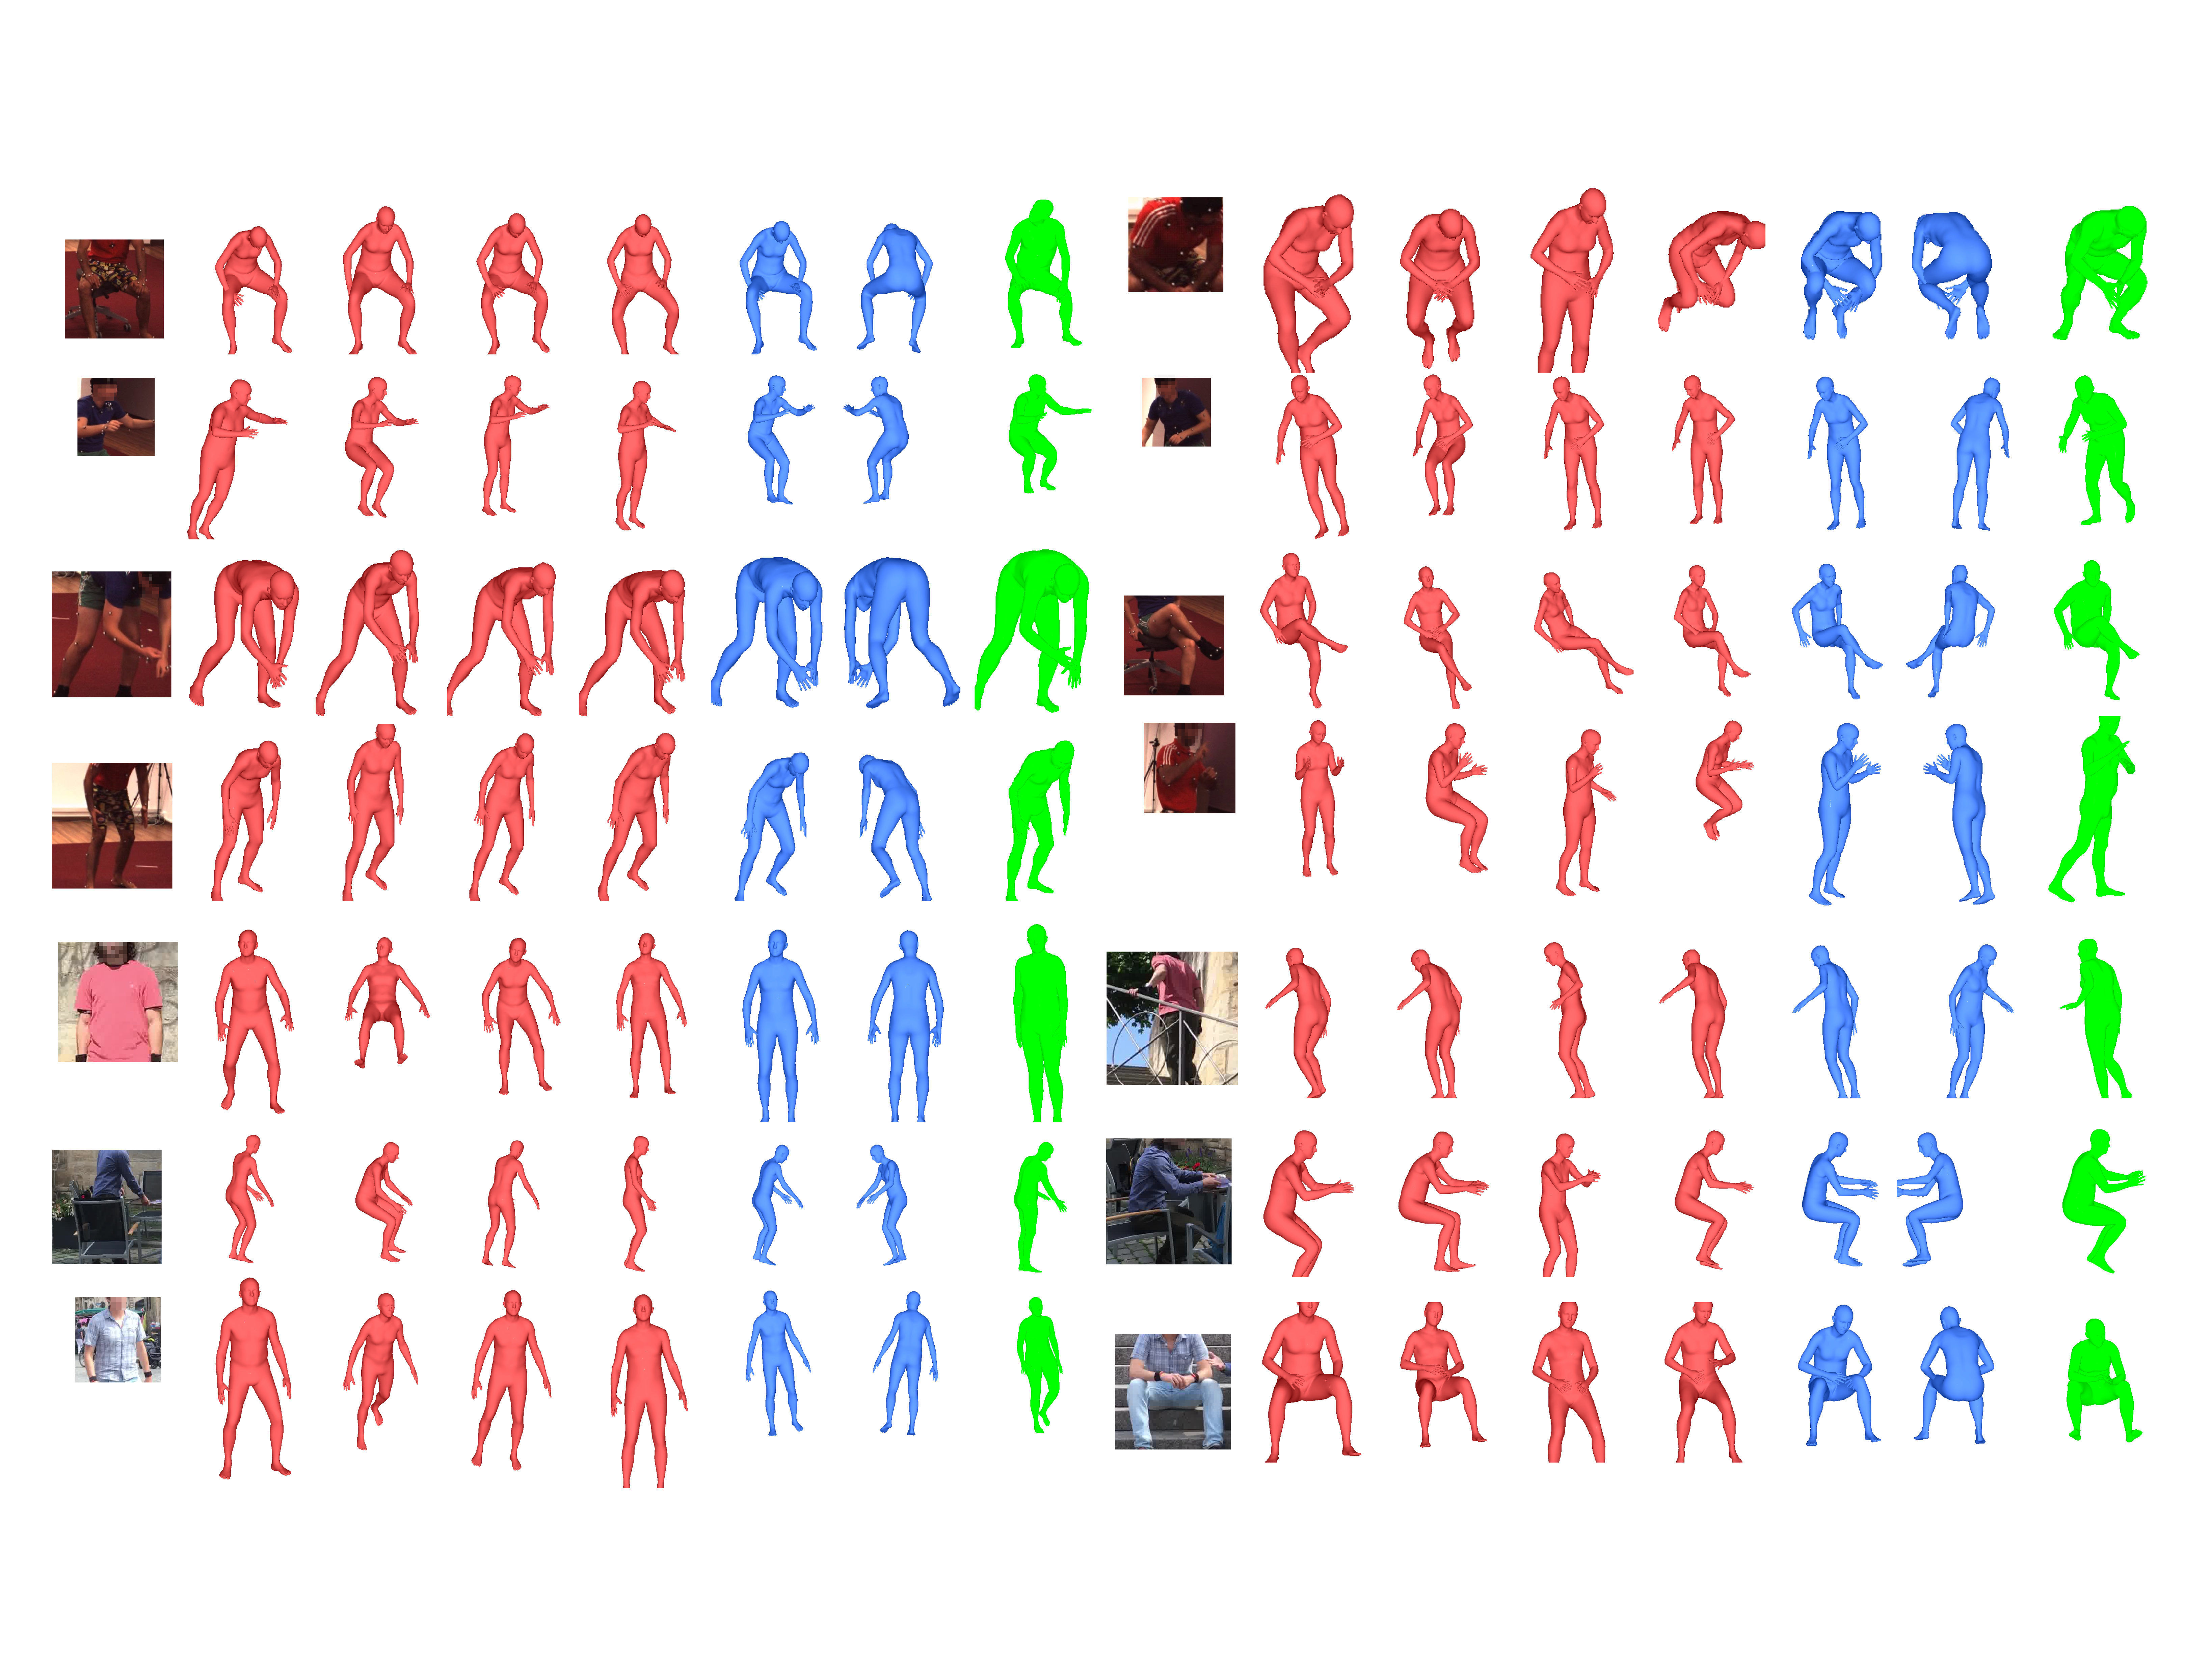
\includegraphics[trim=0.4cm 1cm 8.15cm 1cm,clip,width=0.95\linewidth]{exps/qual_results_all/qualfigs_3.png}
    }

% }
% \vspace{-1.15cm}
\caption{%
    \textbf{Qualitative results from $n=5$ quantization on monocular mesh recovery on AH36m and A3DPW.} 
    From left to right, each group of figures depicts the input ambiguous image, five network hypotheses with the closest to the ground truth in blue, and the ground truth pose in green.
    }\label{fig:qual_results_all}
\end{figure}


\begin{figure}[t]
% \def\bb{\rule{2in}{0pt}\rule{0pt}{1in}}
\centering
% \resizebox{.95\linewidth}{!}{
    \center{
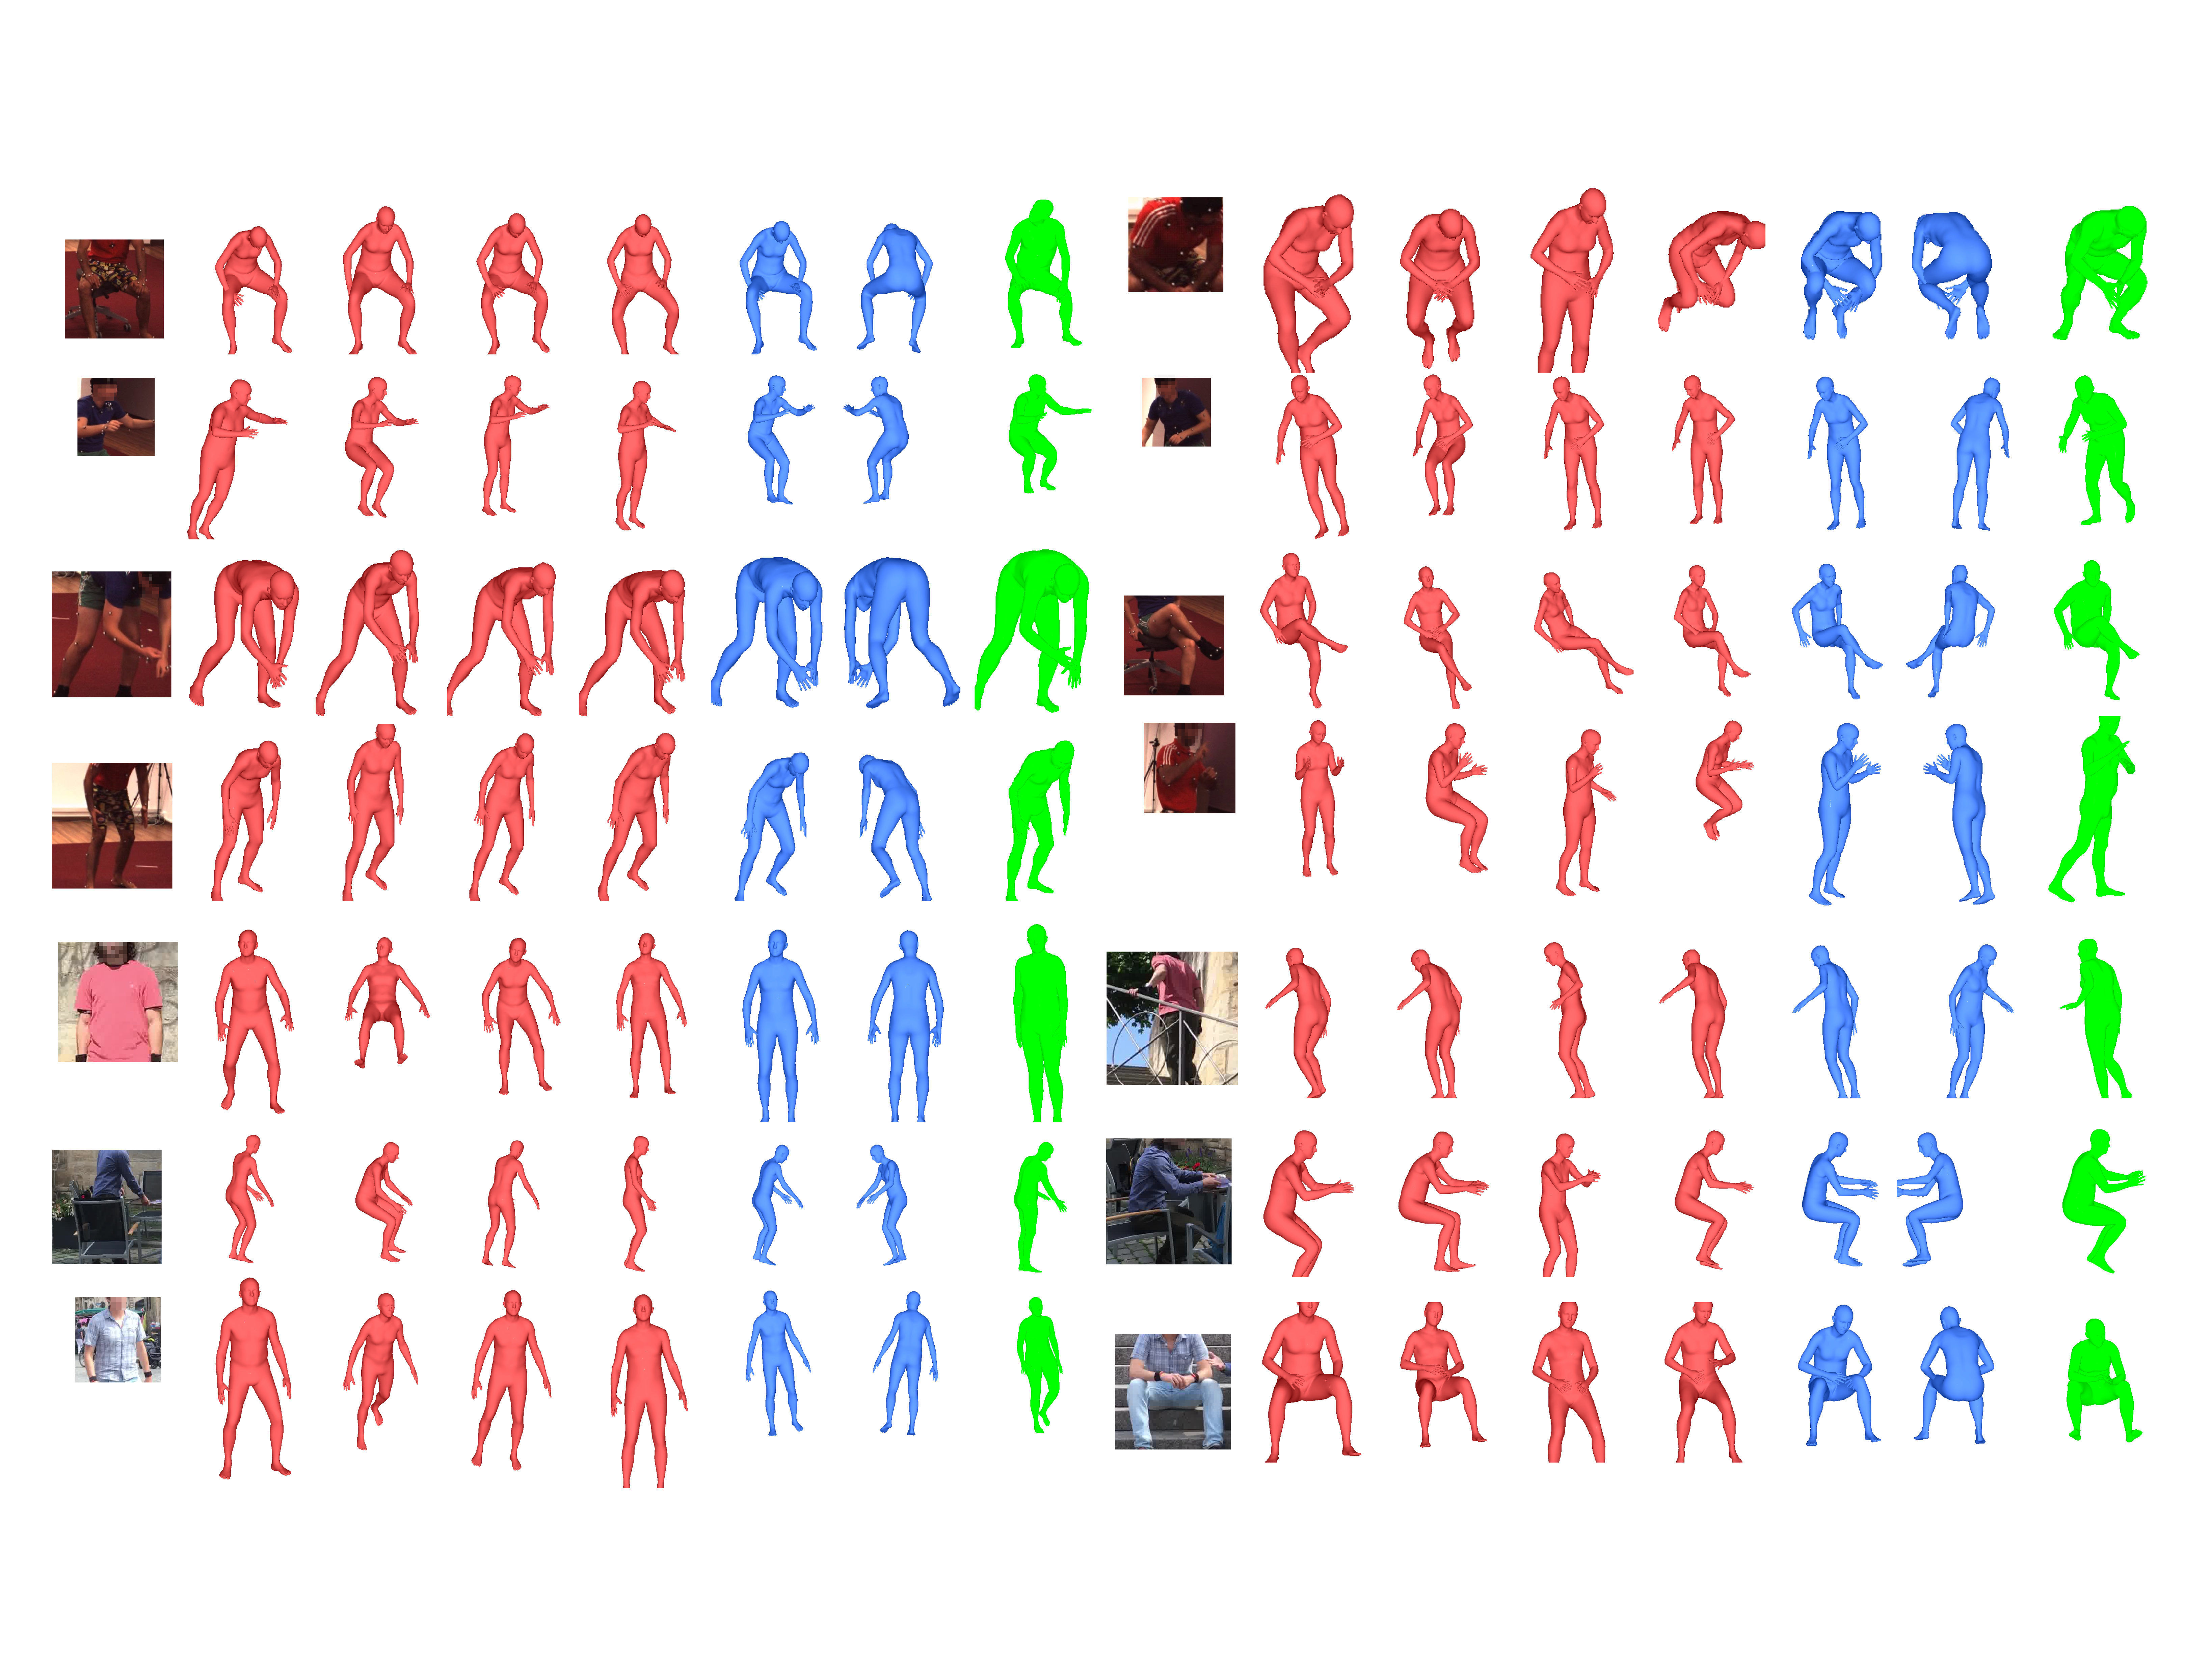
\includegraphics[trim=8.15cm 1cm 0.4cm 1cm,clip,width=0.95\linewidth]{exps/qual_results_all/qualfigs_3.png}
    }
% }
% \vspace{-1.15cm}
\caption{%
    \textbf{Qualitative results from $n=5$ quantization on monocular mesh recovery on AH36m and A3DPW (continued).} 
    From left to right, each group of figures depicts the input ambiguous image, five network hypotheses with the closest to the ground truth in blue, and the ground truth pose in green.
    }\label{fig:qual_results_all2}
\end{figure}


% TODO: integrate
\section{Results on MS-COCO} \label{s:supp_qual}
In addition to the experiments with quantitative evaluation on H36m, AH36m and 3DPW in \cref{s:exp}, in this section, we also provide qualitative results on challenging examples from the MS-COCO dataset~\cite{lin2014microsoft}.

% \vspace{-5cm}
\begin{figure}[t]
% \def\bb{\rule{2in}{0pt}\rule{0pt}{1in}}
\centering
% \resizebox{.95\linewidth}{!}{
{\includegraphics[width=1.0\linewidth,trim=80 0 80 0,clip]{exps/qual_results_sup/qualfigs_coco.png}}
% }
\vspace{-1cm}
\caption{%
    \textbf{Qualitative results on monocular mesh recovery on MS-COCO} 
    From left to right, each group of figures depicts the input image with three hypotheses of our network. Note that no 3D ground truth exists for this dataset.
    }\label{fig:h36m_qual_coco}
\end{figure}

% THIS STUFF ISN'T VALID. TRAINED IN DIFFERENT WAY.
% \section{Results on COCO and 3DPW}
% In addition to the experiments with quantitative evaluation on H36m and AH36m in \cref{s:exp}, in this section, we also provide qualitative results on the MS-COCO dataset~\cite{lin2014microsoft}. Differently from the (A){}H36m, here we train on the SMPL training annotations on MS-COCO provided by the authors of~\cite{kolotouros19learning}. We train on the training image set and test on the MS-COCO val images. Since our method requires 2D keypoints as input, at test time, the network takes as input the 2D keypoint detections from the OpenPose keypoint detector~\cite{cao2018openpose}.

% \Cref{fig:coco_unamb,fig:amb_coco} contain example monocular SMPL predictions on the val set of MS-COCO\@.
% Additionally, in \cref{fig:3dpw_v2,fig:3dpw_v2_2} we provide example results of the COCO-trained model on several videos of the test set of 3DPW~\cite{vonmarcard2018recovering}. We can observe that the best SMPL hypothesis is correctly aligned with the input image, and that the whole set of image hypotheses correctly covers the space of pose ambiguities.

% \begin{figure*}[h!]
    \centering

    \includegraphics[width=0.24\linewidth]{exps/coco_figures/0000.pdf}
    \includegraphics[width=0.24\linewidth]{exps/coco_figures/0001.pdf}
    \includegraphics[width=0.24\linewidth]{exps/coco_figures/0002.pdf}
    \includegraphics[width=0.24\linewidth]{exps/coco_figures/0003.pdf}
    
    \includegraphics[width=0.24\linewidth]{exps/coco_figures/0021.pdf}
    \includegraphics[width=0.24\linewidth]{exps/coco_figures/0005.pdf}
    \includegraphics[width=0.24\linewidth]{exps/coco_figures/0006.pdf}
    \includegraphics[width=0.24\linewidth]{exps/coco_figures/0023.pdf}
    
    \includegraphics[width=0.24\linewidth]{exps/coco_figures/0008.pdf}
    \includegraphics[width=0.24\linewidth]{exps/coco_figures/0009.pdf}
    \includegraphics[width=0.24\linewidth]{exps/coco_figures/0010.pdf}
    \includegraphics[width=0.24\linewidth]{exps/coco_figures/0011.pdf}
    
    \includegraphics[width=0.24\linewidth]{exps/coco_figures/0026.pdf}
    \includegraphics[width=0.24\linewidth]{exps/coco_figures/0013.pdf}
    \includegraphics[width=0.24\linewidth]{exps/coco_figures/0027.pdf}
    \includegraphics[width=0.24\linewidth]{exps/coco_figures/0015.pdf}
    
    \includegraphics[width=0.24\linewidth]{exps/coco_figures/0029.pdf}
    \includegraphics[width=0.24\linewidth]{exps/coco_figures/0017.pdf}
    \includegraphics[width=0.24\linewidth]{exps/coco_figures/0018.pdf}
    \includegraphics[width=0.24\linewidth]{exps/coco_figures/0019.pdf}

    \caption{%
    \textbf{Qualitative results on COCO validation set.} 
    For each sample we show the input on the left and the Min-of-M result from our $M=3$ model on the right.
    }\label{fig:coco_unamb}
\end{figure*}
% \begin{figure*}[ht!]
    \centering

    \includegraphics[width=0.49\linewidth]{exps/coco_amb_figures/0008.pdf}%
    \includegraphics[width=0.49\linewidth]{exps/coco_amb_figures/0005.pdf}

    \includegraphics[width=0.49\linewidth]{exps/coco_amb_figures/0002.pdf}%
    \includegraphics[width=0.49\linewidth]{exps/coco_amb_figures/0003.pdf}

    \includegraphics[width=0.49\linewidth]{exps/coco_amb_figures/0011.pdf}%
    \includegraphics[width=0.49\linewidth]{exps/coco_amb_figures/0020.pdf}

    \includegraphics[width=0.49\linewidth]{exps/coco_amb_figures/0006.pdf}%
    \includegraphics[width=0.49\linewidth]{exps/coco_amb_figures/0007.pdf}

    \includegraphics[width=0.49\linewidth]{exps/coco_amb_figures/0019.pdf}%
    \includegraphics[width=0.49\linewidth]{exps/coco_amb_figures/0009.pdf}

    \includegraphics[width=0.49\linewidth]{exps/coco_amb_figures/0000.pdf}%
    \includegraphics[width=0.49\linewidth]{exps/coco_amb_figures/0014.pdf}

    \caption{%
    \textbf{Multi-hypothesis results on COCO validation set.}
    For each sample we show the input on the left and results from our $M=5$ model on the right.
    }\label{fig:amb_coco}
\end{figure*}


\subsubsection{Ablation study.}
We further conduct an ablative study on 3DPW that removes components of our method and measures the incurred change in performance. More specifically, we: 1) ablate the hypothesis reprojection loss; 2) set $p(X|I)=\text{Uniform}$ in \cref{e:loss-quant}, effectively removing the normalizing flow component and executing unweighted K-Means in $n$-quantized-best-of-$M$. \Cref{tab:tab_abl} demonstrates that removing both contributions decreases performance, validating our design choices.

\subsubsection{Performance analysis.}
A single inference pass takes on average 0.14s per image on NVIDIA V100 GPU.



% Finally, validating the contributions of our method, the ablation study in \cref{tab:abl_ambi} 
% reports significant drops in performance after removing each of the proposed components of our approach.
% The results in \cref{tab:abl_unambi} demonstrate that removing both contributions significantly decreases performance.
% Removing normalizing flow has a significant impact for $M>1$ while being on par with the no-flow baseline for $M=1$.
% This is expected since our improved modelling of ambiguities in the flow-regularized space can only be effective for $M>1$.

% \input{tab_base_h36m_std}

% \input{tab_base_3dpw_std}

% \input{tab_base_h36m_amb}




% --------------------- SCRATCH BELOW ---------------------
% --------------------- SCRATCH BELOW ---------------------
% --------------------- SCRATCH BELOW ---------------------
% --------------------- SCRATCH BELOW ---------------------
% --------------------- SCRATCH BELOW ---------------------
% --------------------- SCRATCH BELOW ---------------------
% --------------------- SCRATCH BELOW ---------------------
% --------------------- SCRATCH BELOW ---------------------
% --------------------- SCRATCH BELOW ---------------------
% --------------------- SCRATCH BELOW ---------------------
% --------------------- SCRATCH BELOW ---------------------


% \subsection{Standard human mesh recovery}\label{s:exp_sota_unambi}

% First, in order to validate our approach, we compare with the state-of-the-art on the standard H36M dataset using the \MPJPE, \RE and \SE metrics.


% % \input{tab_sota_h36m_std}

% \subsection{Multi-pose estimation} \label{s:exp_mutlipose}

% Here, we focus on the main evaluation that assesses the ability of the benchmarked approaches to cover the set of plausible poses given a single input image.

% \paragraph{Multi-hypothesis baselines.}

% Our flow-based method is compared to two multi-pose prediction baselines. \textbf{SMPL-MDN} builds on our keypoint-conditioned trunk architecture and, following~\cite{li19generating}, outputs parameters of a mixture density model over the set of SMPL log-rotation pose parameters.
% Since a na\"{\i}ve implementation of the MDN model that only optimizes the log-likelihood of the mixture of log-rotations leads to very poor performance ($\approx$ 200mm \MPJPE-$M=3$), we introduce several improvements.
% The most critical of these is the addition of the total loss \cref{e:loss-total}, which allows direct optimization over the 3D joint and dense vertex error. We find this is necessary to obtain competitive performance.
% Full description of SMPL-MDN has been deferred to the supplementary.

% We further introduce \textbf{SMPL-CVAE}, which is a variant of the conditional variational autoencoder~\cite{sohn2015cvae} combined with our trunk MLP network.
% SMPL-CVAE consists of an encoding network that maps a ground truth SMPL mesh $V$ to a gaussian vector $z$ which is fed together with an encoding of the conditioning information (a list of 2D keypoints in our case) to generate a mesh $V'$ such that $V' \approx V$.
% The space of Gaussian vectors $z$ is further regularized so that, during test stage, we can replace the ground-truth conditioned encoder network with a random sampler of $z \sim \mathcal{N}(0, 1)$.
% This way, for a given test image, we randomly sample $M$ plausible human meshes that are evaluated with \MPJPE-$M$.
% A more detailed explanation of SMPL-CVAE is in the supplementary.

% \input{fig-best}
% \input{fig-qualresults}
%\input{fig-mdn-vs-ours}

% % place holder
% \begin{figure*}
%     \centering
%     \fbox{\makebox(460,100){}}
%     \caption{Best in blue, GT right most. \label{fig:h36m_qual}}
% \end{figure*}
% \newcommand{\vspacekill}{\vspace{-0.4cm}}
\newcommand{\flowfig}[1]{
\includegraphics[width=0.1\linewidth,trim=200 200 200 200,clip]{exps/flow_samples/sample_#1.png}}
% final figure
\begin{figure*}
    \centering
    \flowfig{00004}%
    \flowfig{00016}%
    \flowfig{00031}%
    \flowfig{00038}%
    \flowfig{00041}%
    \flowfig{00050}%
    \flowfig{00054}%
    \flowfig{00061}%
    \flowfig{00078}%
    \caption{%
    \textbf{Example samples from the normalizing flow} 
    $f: X \mapsto z;~ p(z) \sim \mathcal{N}(0,1)$,
    trained on a dataset of ground truth 3D SMPL control skeletons $\{X_1, ..., X_N\}$.
    }\label{fig:nf_samples}
\end{figure*}

% % \rk{Carefuly explain the deletion of keypoints instead of cropping the image}

% The results in \cref{tab:tab_base_h36m_std} reveal that our approach outperforms both baselines across all numbers of used modes $M$ by a significant margin.
% For SMPL-CVAE, we found that the encoding network often ``cheats'' by transporting all information about the ground truth, instead of only encoding the modes of ambiguity.
% The reason for a lower performance of SMPL-MDN is probably the representation of the probability in the space of log-rotations, rather in the space of vertices.
% Modelling the MDN in the space of model vertices would be more convenient due to being more relevant to the final evaluation metric that aggregates per-vertex errors, however, fitting such high-dimensional (dim=$6890 \times 3$) Gaussian mixture is prohibitively costly. Conversely, our approach is capable of modelling the ambiguities in the log-rotation space while being directly connected to the vertex space via the bijective normalizing flow transformation.

% \input{tab_base_h36m_std}

% \input{tab_base_3dpw_std}

% \paragraph{Ablation study.}

% In order to evaluate the contribution of the individual components of our approach, we conduct an ablative study that removes the components and measures the incurred change in performance.
% To this end we evaluate two variants of our method: (1)~\textbf{Ours w/o Mode Re-proj.} that removes the mode re-projection loss from \cref{e:loss-ri} and; (2)~\textbf{Ours w/o Flow.} which ablates the normalizing flow head.

% % \input{tab_abl_unambi}

% The results in \cref{tab:abl_unambi} demonstrate that removing both contributions significantly decreases performance.
% Removing normalizing flow has a significant impact for $M>1$ while being on par with the no-flow baseline for $M=1$.
% This is expected since our improved modelling of ambiguities in the flow-regularized space can only be effective for $M>1$.

% \subsection{Human mesh recovery on ambiguous H36M}

% We finally turn our attention towards a challenging evaluation on AH36M that exhibits a much higher amount of prediction uncertainty.
% Since, in the previous section, we have demonstrated that predicting shape from 2D keypoint locations leads to a competitive performance, we restrict the evaluation on the AH36M to architectures that take 2D keypoints as input.
% As the main baselines, we  take SMPL-CVAE and SMPL-MDN\@.
% Within this section, all methods have been both trained and tested on AH36M.

% The results in \cref{tab:baseline-ambi} demonstrate that our method outperforms SMPL-CVAE and SMPL-MDN across all values of $M$ on all considered metrics.
% Finally, validating the contributions of our method, the ablation study in \cref{tab:abl_ambi} reports significant drops in performance after removing each of the proposed components of our approach.

% \input{tab_base_h36m_amb}

% \input{tab_multi_baselines_ambi}
% \input{tab_abl_ambi}

%\subsection{Qualitative results}

%\paragraph{Monocular 3D body reconstruction.}

%Qualitative results on the ambiguous H36M dataset depicting a comparison between the SMPL-MDN and our method are in \cref{fig:mdn-vs-ours}.
%We observe that our method exhibits increased diversity among predicted hypotheses than SMPL-MDN.



% \input{fig_quali.tex}

% \paragraph{Samples from the normalizing flow.} In \cref{fig:flow_samples}, we show the random samples produced by the normalizing flow head of our model. Here, we observe that the normalizing flow model is able to both restrict its samples to plausible human poses, while covering a large set of possible body articulations.

\section{Conclusions}\label{s:conc}

In this work, we have explored a seldom visited problem of representing the set of plausible 3D meshes corresponding to a single ambiguous input image of a human.
To this end, we have proposed a novel method that trains a single multi-hypothesis best-of-$M$ model and, using a novel $n$-quantized-best-of-$M$ strategy, allows to sample an arbitrary number $n<M$ of hypotheses.

Importantly, this proposed quantization technique leverages a normalizing flow model, that effectively filters out the predicted hypotheses that are unnatural.
Empirical evaluation reveals performance superior to several strong probabilistic baselines on Human36M, its challenging ambiguous version, and on 3DPW. Our method encounters occasional failure cases, such as when tested on individuals with unusual shape (e.g. obese people), since we have very few of these examples in the training set. Tackling such cases would make for interesting and worthwhile future work.  